%\setcounter{chapter}{31}
\chapter{Inference in graphical models}
\label{chapt:InferenceInGraphicalModels}

\reviewcomment{Material from this chapter is now merged into "graphical_models.tex" chapter file.}


Given a probabilistic graphical model and observations, we want to estimate the states of 
the unobserved variables. For example, given image
observations, we want to estimate the pose of the person.
The belief propagation algorithm lets us do that efficiently.


Recall the Bayesian inference task:  our observations are the
elements of a vector, $\mathbf{y}$, and we seek to infer the probability
$P(\mathbf{x}|\mathbf{y})$ of some scene
parameters, $\mathbf{x}$, given the observations.  By Bayes' rule, we have
\begin{equation}
P(\mathbf{x}|\mathbf{y}) = \frac{P(\mathbf{y}|\mathbf{x}) P(\mathbf{x}) }{P(\mathbf{y}) }
\end{equation}
The {\em likelihood term} $P(\mathbf{y}|\mathbf{x})$ describes how a
rendered scene $\mathbf{x}$ generates observations $\mathbf{y}$.  The {\em
prior probability}, $P(\mathbf{x})$, tells the probability of any given
scene $\mathbf{x}$ occurring.  For inference, we often ignore the denominator,
$P(\mathbf{y})$, called the {\em evidence}, as it is constant with
respect to the variables we seek to estimate, $\mathbf{x}$.

Typically, we make many observations, $\mathbf{y}$, of the variables of some system,
and we want to find the the state of some hidden variable, $\mathbf{x}$, given those
observations.  The posterior probability, $P(\mathbf{x}|\mathbf{y})$, tells
us the probability for any value of the hidden variables, $\mathbf{x}$.
From this posterior probability, we often want some single {\em best} estimate for $\mathbf{x}$,
denoted $\mathbf{\hat{x}}$ and called a point estimate.  

Selecting the best estimate $\mathbf{\hat{x}}$ requires specifying a
penalty for making a wrong guess. If we penalize all wrong answers
equally, the best strategy is to guess the value of  $\mathbf{x}$ that maximizes
the posterior probability, $P(\mathbf{x}|\mathbf{y})$ (because any other
explanation $\mathbf{\hat{x}}$ for the observations $\mathbf{y}$  would be
less probable).  That is called the MAP estimate, for {\em maximum a 
  posteriori}.

But we may want to penalize wrong answers as a function of how far
they are from the correct answer.  If that penalty function is
the squared distance in $\mathbf{x}$, then the point estimate that
minimizes the average value of that error is called the minimum mean squared error
estimate, or MMSE.  To find this estimate, we seek 
the $\hat{\mathbf{x}}$ that minimizes the squared error, weighted by the probability of each outcome:
\begin{equation}
\hat{\mathbf{x}}_{MMSE} = \mbox{argmin}_{\tilde{\mathbf{x}}} 
\int_{\mathbf{x}} P(\mathbf{x}|\mathbf{y}) (\mathbf{x}-\tilde{\mathbf{x}})'
(\mathbf{x}-\tilde{\mathbf{x}}) d\mathbf{x}
\end{equation} 
Differentiating with respect to $\mathbf{x}$ to solve for the stationary
point, the global minimum for this convex function, we find
\begin{equation}
\hat{\mathbf{x}}_{MMSE} = \int_{\mathbf{x}} \mathbf{x} P(\mathbf{x}|\mathbf{y})  d\mathbf{x}.
\end{equation}
Thus, the minimum mean square error estimate, $\hat{\mathbf{x}}_{MMSE}$,
is the mean of the posterior distribution.  
If $\mathbf{x}$ represents a discretized space, then the
marginalization integrals over $d\mathbf{x}$ become sums over the
corresponding discrete states of $\mathbf{x}$.

For now, we'll assume we seek the MMSE estimate. By the properties of
the multi-variate mean, to find the mean at each variable, or node, in
a network, we can first find the marginal probability at each node,
then compute the mean of each marginal probability.  In other words,
given $P(\mathbf{x} | \mathbf{y})$, we will compute $P(x_i | \mathbf{y})$,
where $i$ is the $i$th hidden node.  From $P(x_i | \mathbf{y})$ it is
simple to compute the posterior mean at node $i$.

For the case of discrete variables, we compute the marginal probability at a node by summing over the states at all the other nodes,
\begin{equation}
    P(x_i | \mathbf{y}) =  \sum_{j  \mbox{\textbackslash} i} \sum_{x_j} 
    P(x_1, x_2, \ldots, x_i, \ldots, x_N|\mathbf{y}),
    \label{eq:discreteMarginalization}
\end{equation}
where the notation $j \mbox{\textbackslash} i$ means "all possible values of j except for j = i".

\section{Simple example of inference in a graphical model}
\label{sect:simpleexample}
To gain intuition, let's calculate the marginal probability for a
simple example.  Consider the three-node Markov chain 
of \ref{fig:chain}, reproduced here.
\begin{equation}
\centerline{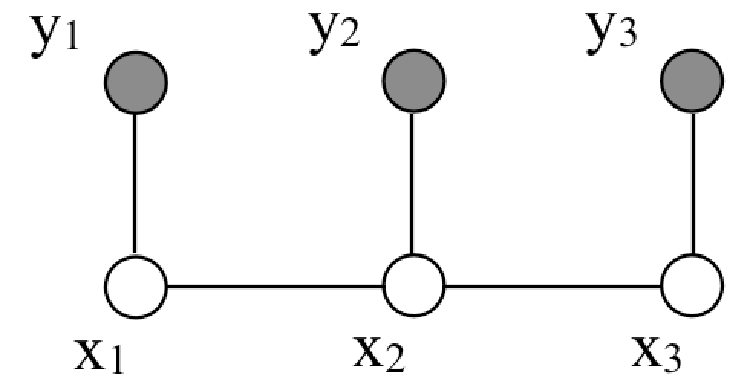
\includegraphics[width=0.36\linewidth]{figures/graphical_models/x1x2x3y1y2y3.pdf}} 
\label{fig:chain2}
\end{equation}
Vision tasks this can apply to include modeling the probability of a pixel
belonging to an object edge, given the evidence, observations $\mathbf{y}$, at a point and two
neighboring locations.  The inferred states $\mathbf{x}$ could be a label
indicating the presence of an edge.

We seek to marginalize the joint probability in order to
find the marginal probability at node 1, $P(x_1|\mathbf{y})$, given
obervations $y_1$, $y_2$, and $y_3$, which we denote as $\mathbf{y}$.
We have, assuming the nodes have discrete states,
\begin{equation}
P(x_1|\mathbf{y}) = \sum_{x_2} \sum_{x_3}  P(x_1, x_2, x_3|\mathbf{y})
\label{eq:3chain}
\end{equation}

Here's the main point:  If we knew nothing about the structure of
the joint probability $P(x_1, x_2, x_3|\mathbf{y})$, the computation would require
$|x|^3$ computations: a double-sum over all $x_2$ and $x_3$ states must
be computed
for each possible $x_1$ state.  (We're denoting the number of states of any of the $x$
variables as $|x|$).  In the more general case, for a Markov chain of
$N$ nodes, we would need $|x|^N$ summations to compute the desired
marginal at any node of the chain.  Such a computation quickly
becomes intractable as $N$ grows.

But we can exploit the model's structure to avoid the
exponential growth of the computation with $N$.
Substituting the joint probability, from the graphical model, into the
marginalization equation, Eq.~(\ref{eq:3chain}), gives
\begin{equation}
P(x_1|\mathbf{y}) = 
\frac{1}{P(\mathbf{y})} \sum_{x_2} \sum_{x_3}  
\phi_{12}(x_1, x_2)  \phi_{23}(x_2, x_3) \psi_{1}(y_1, x_1) \psi_{2}(y_2, x_2) \psi_{3}(y_3, x_3) 
\label{eq:3chainb}
\end{equation}
This form for the joint probability reveals that not every variable is
coupled to every other one.  We can pass summations
through  variables they don't sum over, letting us compute the
marginalization much more efficiently.  This will make only a small
difference for this short chain, but it makes a huge difference
for longer ones.  So we write
\begin{eqnarray}
P(x_1|\mathbf{y}) 
& = & 
\frac{1}{P(\mathbf{y})} \sum_{x_2} \sum_{x_3}  
\phi_{12}(x_1, x_2)  \phi_{23}(x_2, x_3)
\psi_{1}(y_1, x_1) \psi_{2}(y_2, x_2) \psi_{3}(y_3, x_3)  
\label{eq:before}
\\
& = &
\frac{1}{P(\mathbf{y})}
\psi_{1}(y_1, x_1) 
\sum_{x_2} \phi_{12}(x_1, x_2) \psi_{2}(y_2, x_2) 
\sum_{x_3}   \phi_{23}(x_2, x_3)  \psi_{3}(y_3, x_3)  
\label{eq:after} 
\end{eqnarray}
That factorization of Eq.~(\ref{eq:after}) is the key step:
It reduces the number of terms summed from order $|x|^3$ to order $2
|x|^2$ for this chain, and for a chain of length $N$ chain, from order $|x|^N$ to order $(N-1) |x|^2$, a
huge computational savings for large N.  

The partial sums of
Eq.~(\ref{eq:after}) are named  ``messages'' because they pass information from one node to another.  We call the message from node 3
to node 2, $m_{32}(x_2)  = \sum_{x_3}   \phi_{23}(x_2, x_3)
m_{63}(x_3) $.  The other partial sum is the message from node 2 to
node 1, 
$m_{21}(x_1)   = \sum_{x_2} \phi_{12}(x_1, x_2)  m_{52}(x_2)  
m_{32}(x_2) $.
Note that the messages are always messages about
the states of the node that the message is being sent {\em to}--the
arguments of the message $m_{ij}$ are the states $x_j$ of node $j$.  The algorithm corresponding to Eq.~(\ref{eq:after}) is called {\em belief propagation}.

Eq.~(\ref{eq:after}) gives us the marginal probability at node 1.  To
find the marginal probability at another node, you 
can write out the sums over variables needed for that node, pass the
sums through factors in the joint probability that they don't operate
on, to come up with an efficient reorganization of summations analogous to
Eq.~(\ref{eq:after}).  You would find that many
of the summations from marginalization at the node $x_1$  would need
to be recomputed for the marginalization at node $x_2$.  That
motivates storing and reusing the messages, which the belief propagation algorithm does in an optimal way.

\section{Belief propagation (BP)}

For more complicated graphical models, we want to 
replace the manual factorization
with an automatic procedure for identifying the
computations needed for marginalizations and to 
cache them efficiently.  Belief propagation does that by
identifying those reusable sums, the ``messages''. 

\begin{figure}
\centerline{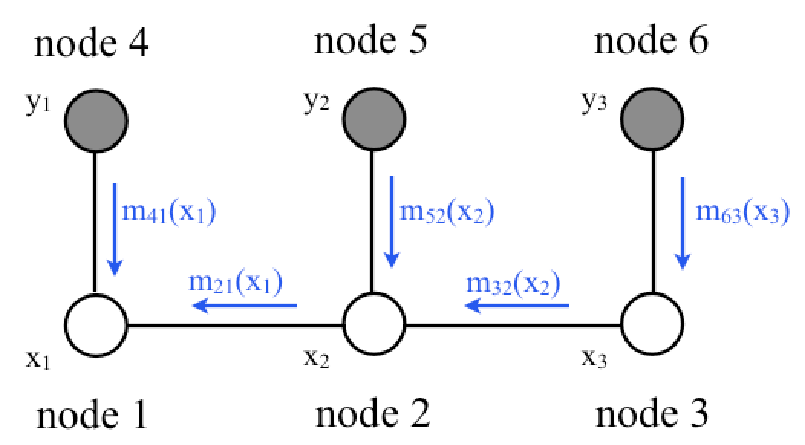
\includegraphics[width=0.60\linewidth]{figures/graphical_models/3bpc.pdf}} 
\caption{Summary of the messages (partial sums) for a simple belief propagation example.} 
\label{fig:3bpc}
\end{figure}

\subsection{Derivation of message-passing rule}
\label{sect:bpRules}

We'll describe belief propagation (BP) only for the special case of
graphical models with pairwise potentials.  
The clique potentials between neighboring nodes are $\psi_{ij}(x_j, x_i)$.
Extensions to higher-order
potentials is straightforward.  (Convert the
graphical model into one with only pairwise potentials.  This can be
done by augmenting the state of some nodes to encompass several nodes,
until the remaining nodes only need pairwise potential functions in
their factorization of the joint probability.)  You can find formal
derivations of belief propagation in \cite{Jordan98,Koller2009}.

Consider Fig.~\ref{fig:bpmotivator2}, showing a section of a general network with pair-wise potentials.  There is a network of $N+1$
nodes, numbered 0 through $N$ and we will marginalize over nodes
$x_1 \ldots x_N$.  Fig.~\ref{fig:bpmotivator2}~(a) shows the
marginalization equation for a network of variables with discrete states. (For continuous variables, integrals replace the summations). If we assume the nodes form a tree, we can
distribute the marginalization sum
past nodes for which the sum is a constant value to obtain the sums
depicted in Fig.~\ref{fig:bpmotivator2}~(b).  

We define a {\em  belief propagation message}:

{\bf A message $m_{ij}$, from node i to node j, is the sum of the
 probability over all states of all
nodes in the subtree that leaves node $i$ and does not include node $j$.}

Referring to Fig.~\ref{fig:bpmotivator2}, (a) shows the desired
marginalization sum over a network of pairwise cliques. (This approach
can be extended to more general cliques).  
We can pass the summations over node states through nodes that are
constant over those summations, arriving at the factorization shown in
(b).  Remembering that the message from node i to node j is the sum
over the tree leaving node i, we can then read-off the recursive
belief propagation message update rule by inspecting
Fig.~\ref{fig:bpmotivator2}:

To compute the message from node j to node i:
\begin{enumerate}
\item Multiply together all messages coming in to node j, except for
 the message from node i back to node j,
\item Multiply by the pairwise compatibility function $\psi_{ij}(x_i, x_j)$.
\item Marginalize over the variable $x_j$.
\end{enumerate}
These steps are summarized in this equation to compute the message
from node j to node i:
\begin{equation} 
m_{ji}(x_i) = \sum_{x_j} \psi_{ij} (x_i, x_j) 
\prod_{k\in \eta(j) \mbox{\textbackslash}   i} m_{kj}(x_j)
\label{eq:bpupdate}
\end{equation} 
where $\eta(j) \mbox{\textbackslash}   i$ means ``the neighbors of
node j except for node i''.  Figure~\ref{fig:bpdiscrete} shows this
equation in a graphical form.  Any local potential functions
$\phi_{j}(x_j)$ are treated as an additional message into node j, $m_{0j}(x_j) = \phi_{j}(x_j)$.
For the case of continuous variables, the
sum over the states of $x_j$ in Eq.~(\ref{eq:bpupdate}) is replaced by an integral over the
domain of $x_j$.


\begin{figure}
\sublabel{a}{\centerline{
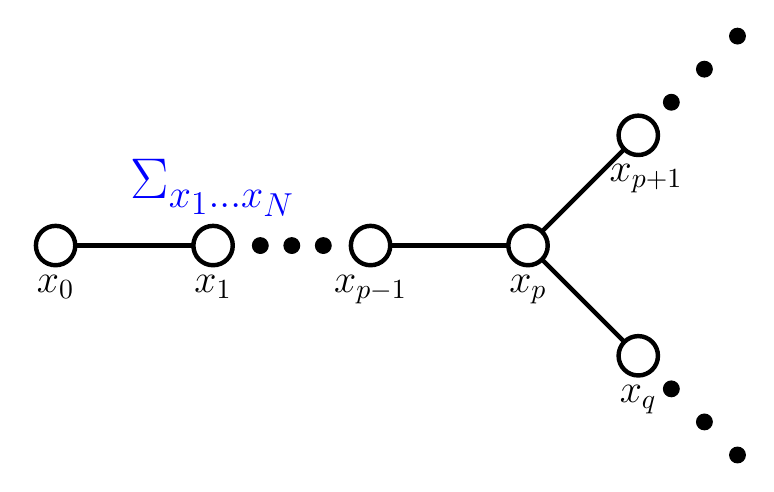
\begin{tikzpicture}
\draw [ultra thick] (-2,0) -- (0,0);
\draw [ultra thick, fill=white] (-2,0) circle [radius=0.25];
\node [below] at (-2,-0.25) {\Large $x_{0}$};
\node [above, blue] at (0,0.25) {\huge $ \Sigma_{x_1 \ldots x_N}$};
\draw [ultra thick, fill=white] (0,0) circle [radius=0.25];
\node [below] at (0, -0.25) {\Large $x_1$};
\draw [fill] (0.6,0) circle [radius=0.1];
\draw [fill] (1,0) circle [radius=0.1];
\draw [fill] (1.4 ,0) circle [radius=0.1];
\draw [ultra thick] (2,0) -- (4,0);
\draw [ultra thick, fill=white] (2,0) circle [radius=0.25];
\node [below] at (2,-0.25) {\Large $x_{p-1}$};
\draw [ultra thick] (4,0) -- (5.4,1.4);
\draw [ultra thick] (4,0) -- (5.4,-1.4);
\draw [ultra thick, fill=white] (4,0) circle [radius=0.25];
\node [below] at (4,-0.25) {\Large $x_p$};
% \draw [fill] (4.6,0) circle [radius=0.1];
% \draw [fill] (5,0) circle [radius=0.1];
% \draw [fill] (5.4 ,0) circle [radius=0.1];
\draw [ultra thick,fill=white] (5.4,1.4) circle [radius=0.25];
\draw [fill] (5.82,1.82) circle [radius=0.1];
\draw [fill] (6.24,2.24) circle [radius=0.1];
\draw [fill] (6.66 ,2.66) circle [radius=0.1];
\node [below] at (5.5,1.15) {\Large $x_{p+1}$};
\draw [ultra thick,fill=white] (5.4,-1.4) circle [radius=0.25];
\node [below] at (5.4,-1.65) {\Large $x_q$};
\draw [fill] (5.82,-1.82) circle [radius=0.1];
\draw [fill] (6.24,-2.24) circle [radius=0.1];
\draw [fill] (6.66 ,-2.66) circle [radius=0.1];
\end{tikzpicture}}}
\sublabel{b}{\centerline{
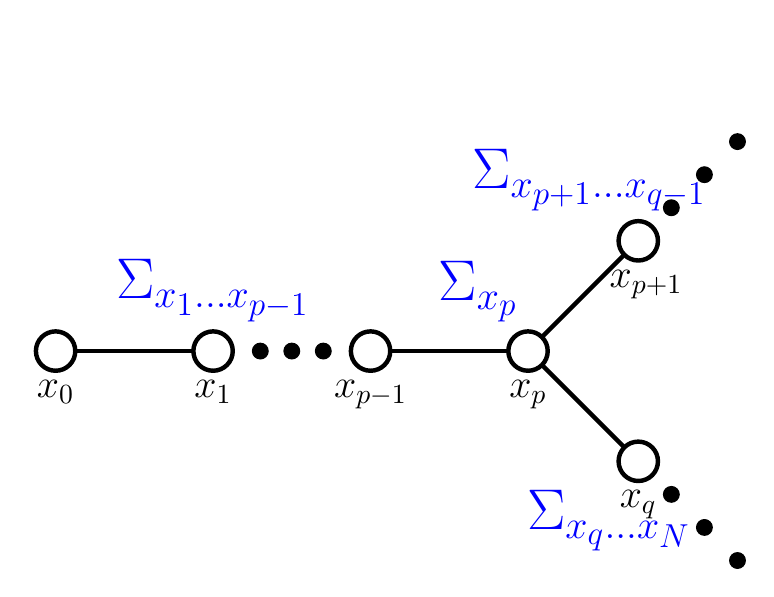
\begin{tikzpicture}
\draw [ultra thick] (-2,0) -- (0,0);
\draw [ultra thick, fill=white] (-2,0) circle [radius=0.25];
\node [below] at (-2,-0.25) {\Large $x_{0}$};
\node [above, blue] at (0,0.25) {\huge $ \Sigma_{x_1 \ldots x_{p-1}}$};
\draw [ultra thick, fill=white] (0,0) circle [radius=0.25];
\node [below] at (0, -0.25) {\Large $x_1$};
\draw [fill] (0.6,0) circle [radius=0.1];
\draw [fill] (1,0) circle [radius=0.1];
\draw [fill] (1.4 ,0) circle [radius=0.1];
\draw [ultra thick] (2,0) -- (4,0);
\draw [ultra thick, fill=white] (2,0) circle [radius=0.25];
\node [below] at (2,-0.25) {\Large $x_{p-1}$};
\draw [ultra thick] (4,0) -- (5.4,1.4);
\draw [ultra thick] (4,0) -- (5.4,-1.4);
\draw [ultra thick, fill=white] (4,0) circle [radius=0.25];
\node [below] at (4,-0.25) {\Large $x_p$};
\node [above left, blue] at (4, 0.25) {\huge $ \Sigma_{x_{p}}$};
\draw [ultra thick,fill=white] (5.4,1.4) circle [radius=0.25];
\draw [fill] (5.82,1.82) circle [radius=0.1];
\draw [fill] (6.24,2.24) circle [radius=0.1];
\draw [fill] (6.66 ,2.66) circle [radius=0.1];
% to add space between the figures
\draw [fill, white] (6.66,4) circle [radius=0.1];
\node [below] at (5.5,1.15) {\Large $x_{p+1}$};
\node [above left, blue] at (6.4, 1.65) {\huge $ \Sigma_{x_{p+1} \ldots x_{q-1}}$};
\draw [ultra thick,fill=white] (5.4,-1.4) circle [radius=0.25];
\node [below] at (5.4,-1.65) {\Large $x_q$};
\node [below left, blue] at (6.2, -1.65) {\huge $ \Sigma_{x_{q} \ldots x_{N}}$};
\draw [fill] (5.82,-1.82) circle [radius=0.1];
\draw [fill] (6.24,-2.24) circle [radius=0.1];
\draw [fill] (6.66 ,-2.66) circle [radius=0.1];
\end{tikzpicture}}}
\caption{Generic example motivating the formula for belief propagation.(a)
  shows the marginalization for a general graph with no loops, focussing on the
  partial sums at note $x_p$.  (b) Shows how the partial sums
  distribute over the nodes.  Note that, by the definition of a message, $m_{p+1,p}$ and $m_{qp}$ correspond to these partial sums over nodes indicated in the graph: 
  $m_{p+1,p} = \sum_{x_{p+1} \ldots x_{q-1}}$ and 
  $m_{qp} = \sum_{x_q \ldots x_N}$.  Marginalization over the states of all nodes leaving node $p$, not including node $p-1$, leads to Eq.~(\ref{eq:bpupdate}) for the belief propagation message passing rule.} 
\label{fig:bpmotivator2}
\end{figure}


\begin{figure}
\centerline{
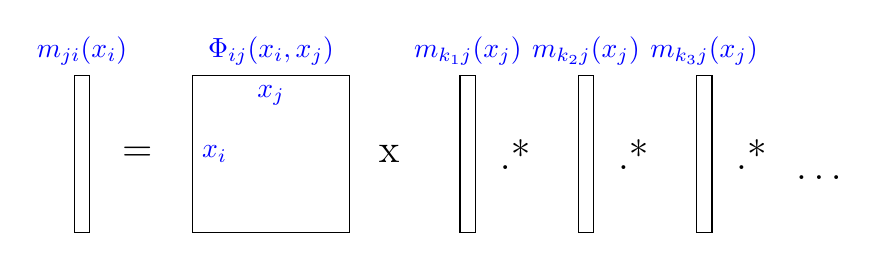
\begin{tikzpicture}
\draw [draw=black]  (-2.8, 2) rectangle (-3, 0);
\node [above, blue] at (-2.9, 2) {$m_{ji}(x_i)$};
\node at (-2.2,1) {\Large  $ =$};
\draw [draw=black]  (-1.5, 2) rectangle (0.5, 0);
\node [above,blue] at (-0.5, 2) {$\Phi_{ij}(x_i, x_j)$};
\node [below, blue] at (-0.5, 2) {$x_j$};
\node [right, blue] at (-1.5, 1) {$x_i$};
\node at (1.0,1) {\Large  $\mbox{x}$};
\draw [draw=black]  (1.9, 2) rectangle (2.1, 0);
\node [above, blue] at (2.0, 2) {$m_{{k_1}j}(x_j)$};
\node at (2.6,1) {\Large  $\mbox{.*}$};
\draw [draw=black]  (3.4, 2) rectangle (3.6, 0);
\node [above, blue] at (3.5, 2) {$m_{{k_2}j}(x_j)$};
\node at (4.1,1) {\Large  $\mbox{.*}$};
\draw [draw=black]  (4.9, 2) rectangle (5.1, 0);
\node [above, blue] at (5.0, 2) {$m_{{k_3}j}(x_j)$};
\node at (5.6,1) {\Large  $\mbox{.*}$};
\node at (6.5,0.7) {\Large  $\mbox{\ldots}$};
\end{tikzpicture}}
\caption{Pictorial depiction of belief propagation message passing
 rules of Eq.~(\ref{eq:bpupdate}),
 showing the vector and matrix shapes.  To send a message from node j to
 node i:  We term-by-term multiply (shown by .*) the messages (column vectors)
 coming in to node j, then matrix multiply (shown by $\mbox{x}$)
the resulting column vector by the compatibility matrix $\Phi_{ij}(x_i, x_j)$ to obtain $m_{ji}(x_i)$.
} 
\label{fig:bpdiscrete}
\end{figure}


As mentioned above, BP messages are partial sums in the
marginalization calculation.  The arguments of messages are always the
state of the node that the message is going to.
(Belief propagation follows the “nosey neighbor rule” (from Brendan Frey, U. Toronto). Every node is a house in some neighborhood. Your nosey neighbor says to you: “given what I've seen myself and everything I’ve heard from my neighbors, here’s what I think is going on inside
your house.” That metaphor made sense to me after my children became teenagers.)


\subsection{Marginal probability}

\begin{figure}
\centerline{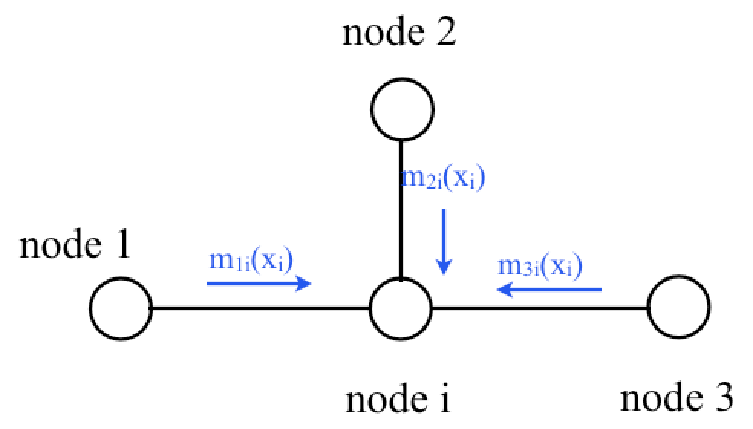
\includegraphics[width=0.48\linewidth]{figures/graphical_models/bpi.pdf}} 
\caption{To compute the marginal probability at node i, we multiply
 together all the incoming messages at that node:  
$P_{i}(x_i) =  \prod_{j\in \eta(i)}  m_{ji}(x_i)$, remembering to
include any local potential terms $\phi_i(x_i)$ as another message.
}
\label{fig:bpi}
\end{figure}
 
The marginal probability at a node i, Eq.~(\ref{eq:discreteMarginalization}), is the sum over the joint probabilities of all states except those of $x_i$.  Because we assume the network has no loops, the conditional
independence structure assures us that marginal probability at a node i is the product of the sum of all states of all nodes in each
sub-tree connected to node i.  (Conditioned on node i, the probabilities within each subtree are independent). Thus the marginal probability at node i
is the product of all the incoming messages:
\begin{equation}
P_{i}(x_i) = \prod_{j\in \eta(i)}  m_{ji}(x_i)
\label{eq:bpmarginal}
\end{equation}
(We include the local clique potential at node i, $\psi_i(x_i)$, as
one of the messages in the product of all messages into node i).


\subsection{Message update sequence}
To find all the messages, how do we invoke the recursive BP update rule, Eq.~(\ref{eq:bpupdate})?  We can apply Eq.~(\ref{eq:bpupdate})
whenever all the incoming messages in the BP update rule are defined.  If there
 are no incoming messages to a node, then its outgoing message is
well-defined in the update rule.  This lets us start the recursive algorithm.

A node can send a message whenever all the incoming messages it needs
have been computed.  We can compute the outgoing messages
from leaf nodes in the graphical model tree, since they have no
incoming messages other than from the node to which they are sending a
message, which doesn't enter in the outgoing message computation.  Two
natural message passing protocols are consistent with that rule:
depth-first update, and parallel update.  In depth-first update, one
node is arbitrarily picked as the root.  Messages are then passed from
the leaves of the tree (leaves, relative to that root node) up to the
root, then back down to the leaves.  In parallel update, at each turn,
every node sends every outgoing message for which it has received all
the necessary incoming messages.  Figure~\ref{fig:men} depicts the
flow of messages for the parallel, synchronous update scheme.

Note that, when computing marginals at many nodes, we re-use messages
with the BP algorithm.  A single message-passing sweep through all the
nodes lets us calculate the marginal at any node (using the
depth-first update rules to calculate the marginal at the root node).
A second sweep from the root node back to all the leaf nodes
calculates all the messages needed to find the marginal probability at
every node.  It takes only twice the number of computations to
calculate the incoming messages to every node as it does to
calculate the incoming messages at a single node.

\begin{figure}
\centerline{
\sublabel{a}{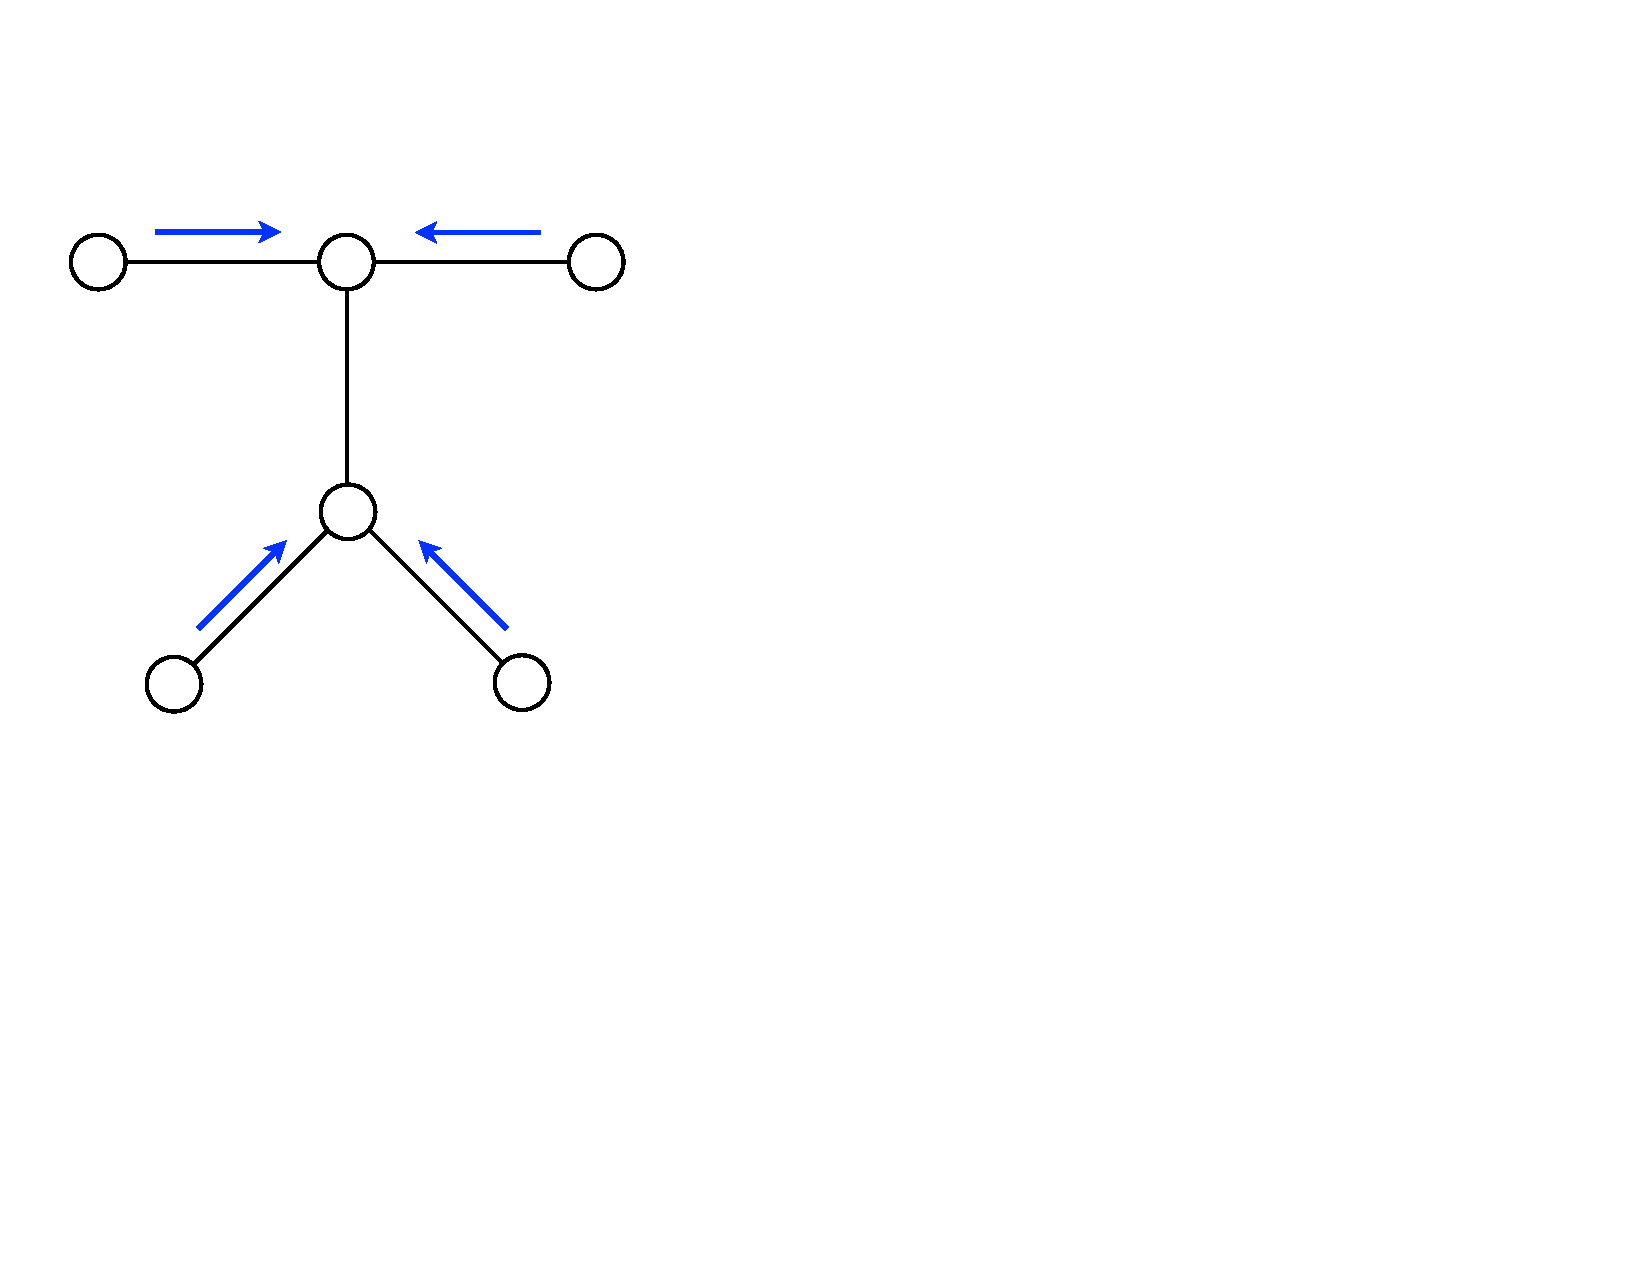
\includegraphics[width=0.20\linewidth]{figures/graphical_models/man1.pdf}}
\sublabel{b}{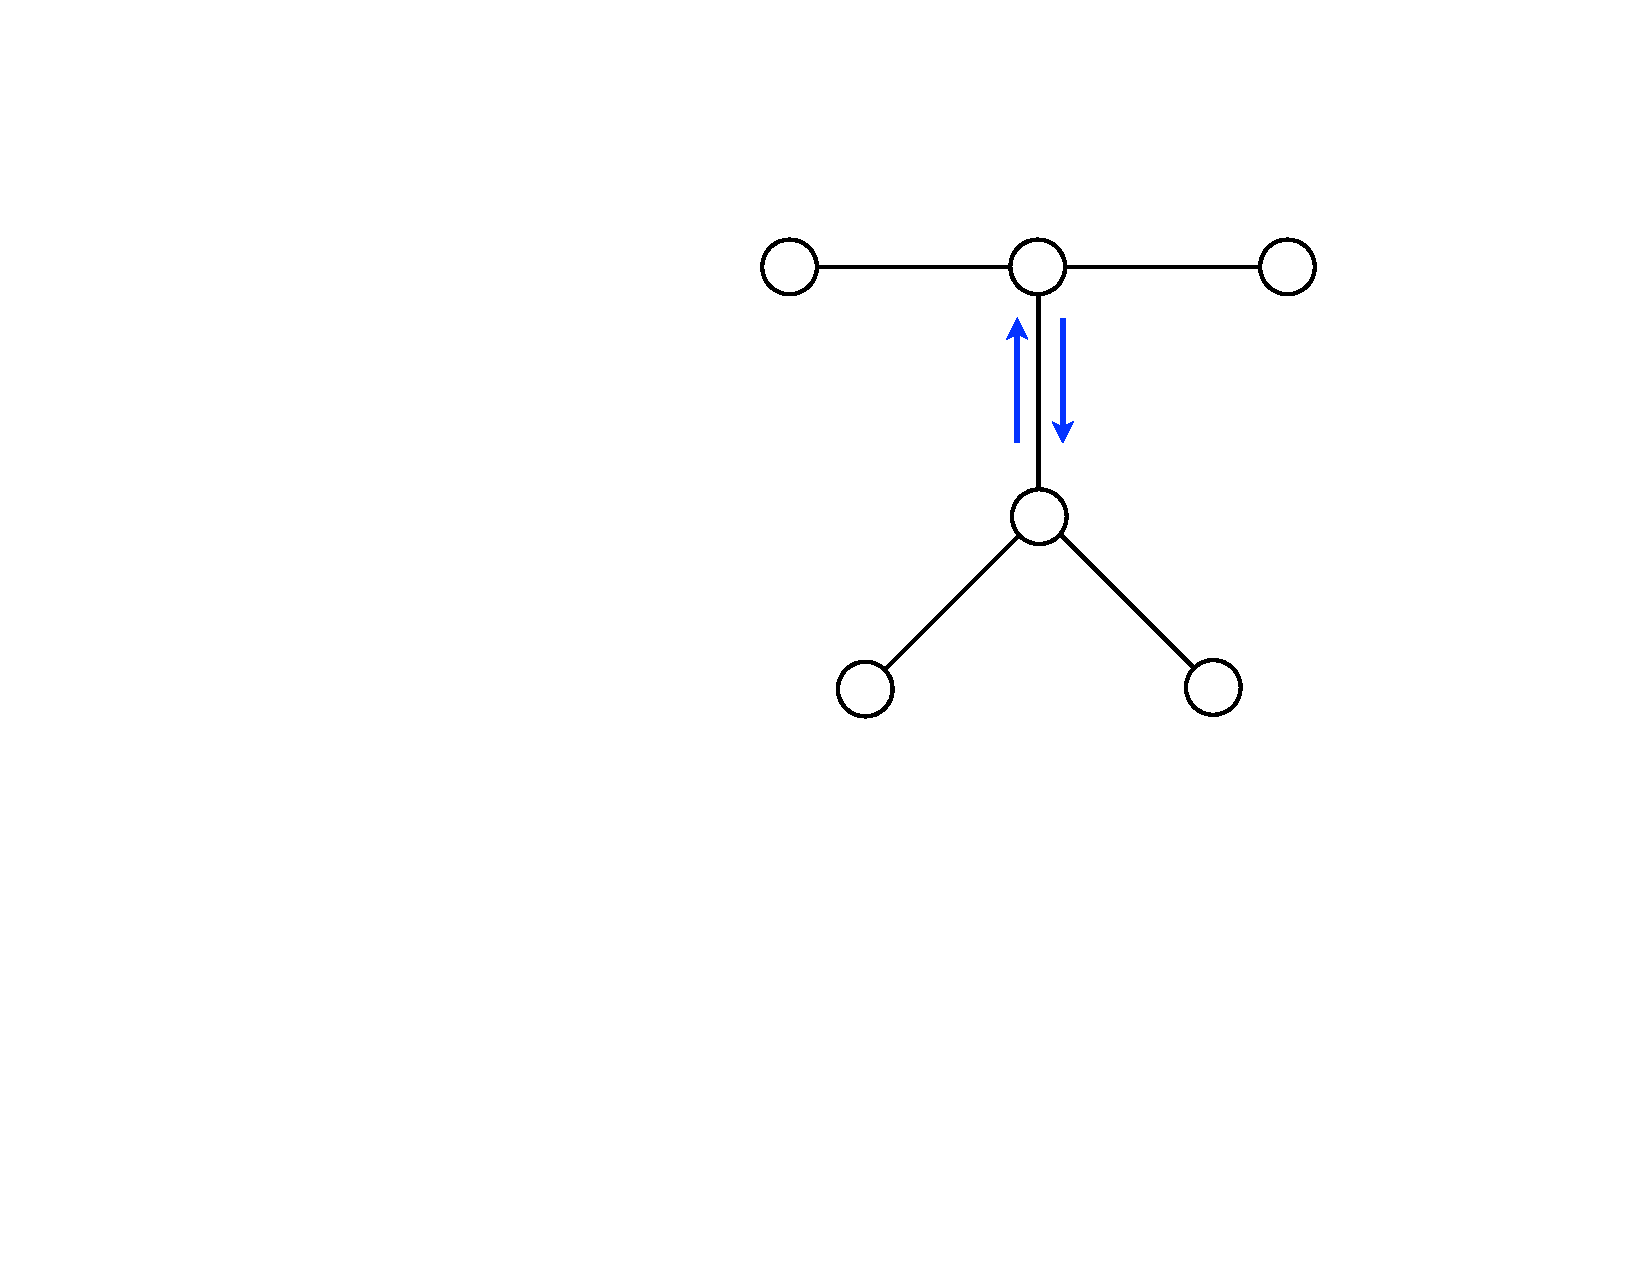
\includegraphics[width=0.20\linewidth]{figures/graphical_models/man2.pdf}}
\sublabel{c}{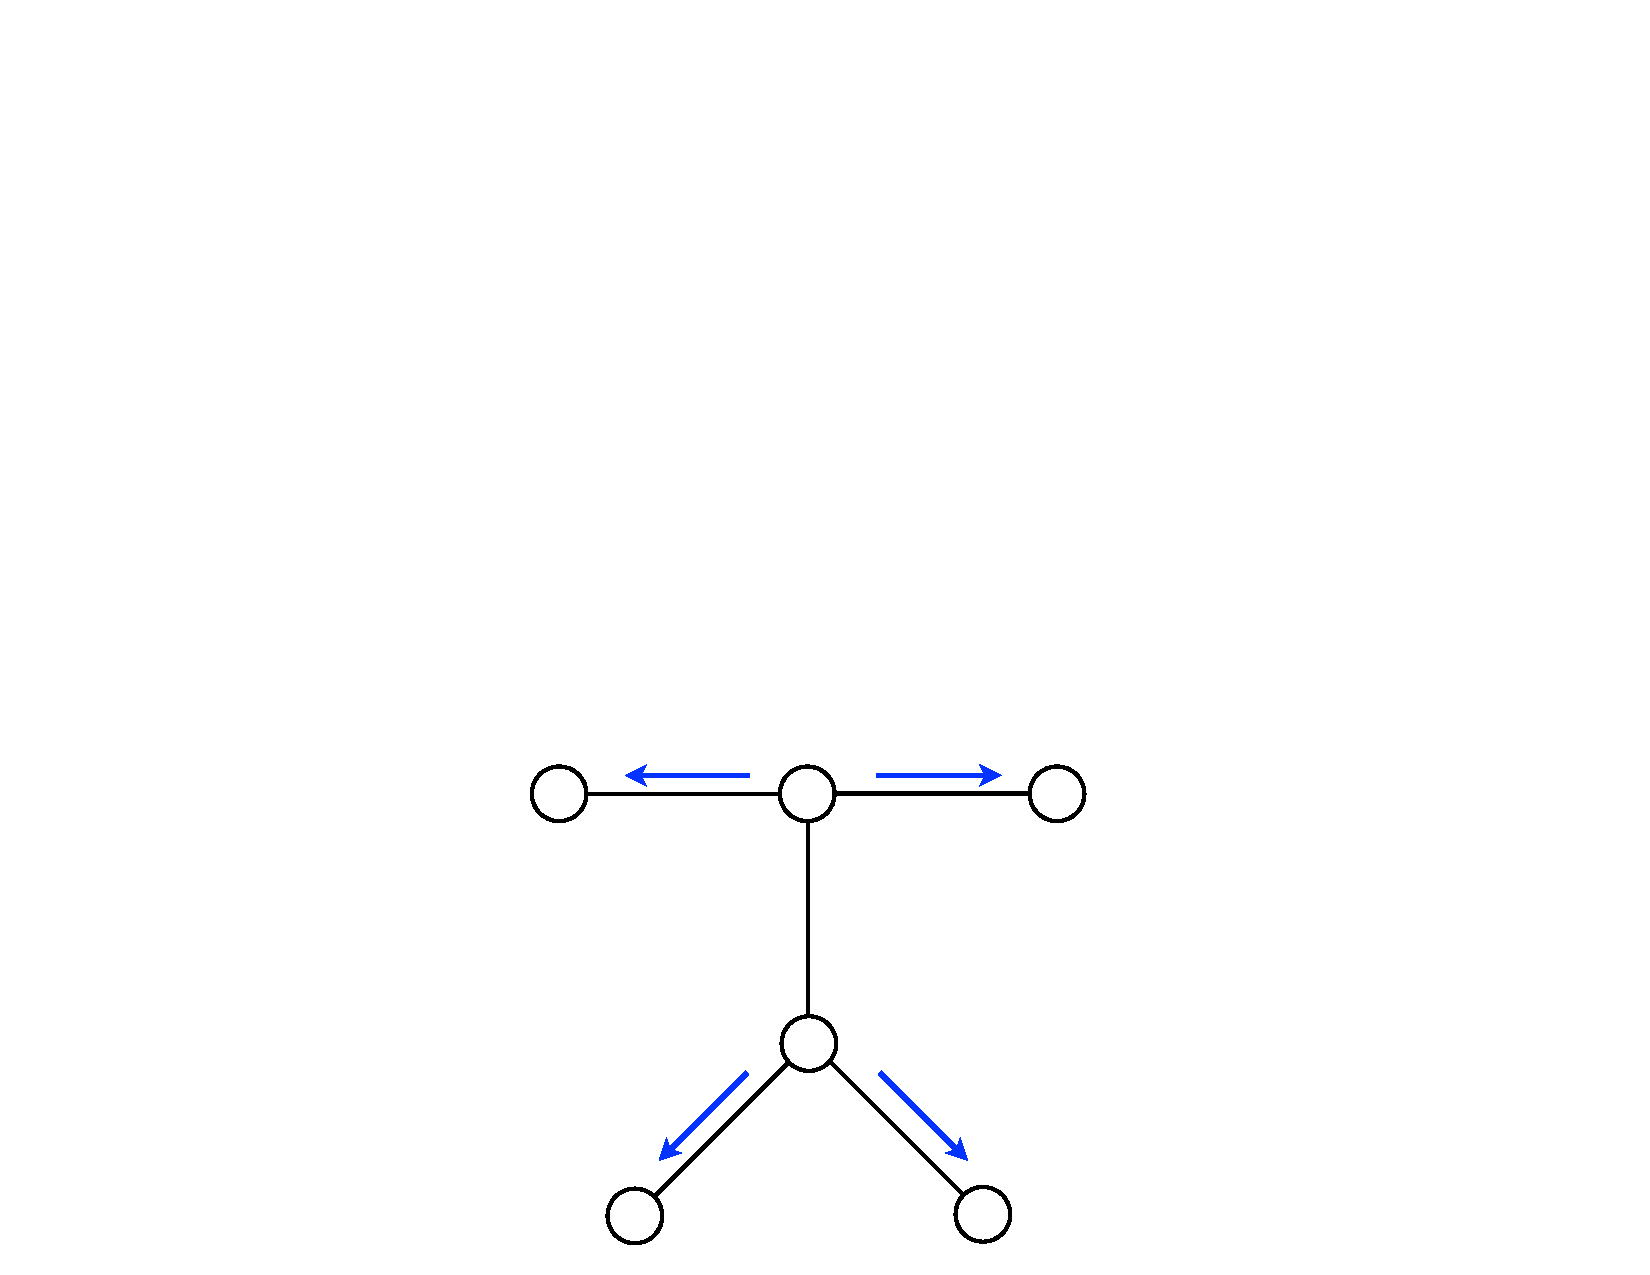
\includegraphics[width=0.20\linewidth]{figures/graphical_models/man3.pdf}}
}
\caption{Example of a {\bf synchronous parallel update schedule} for BP
  message passing.  Whenever any node has the required incoming
  messages needed to send an outgoing message, it does.  (a) At the
  first iteration, only the leaf nodes have the needed incoming
  messages to send an outgoing message (by definition, leaf nodes have
  no links other than the one on which they'll be sending their
  outgoing message, so they have no incoming messages to wait for).   (b) second iteration,
  (c) third iteration.  By the third iteration, every edge has
  messages computed in both directions, and we can now compute the
  marginal probability at every node in the graph.} 
\label{fig:men}
\end{figure}




\begin{figure}
\centerline{
\sublabel{a}{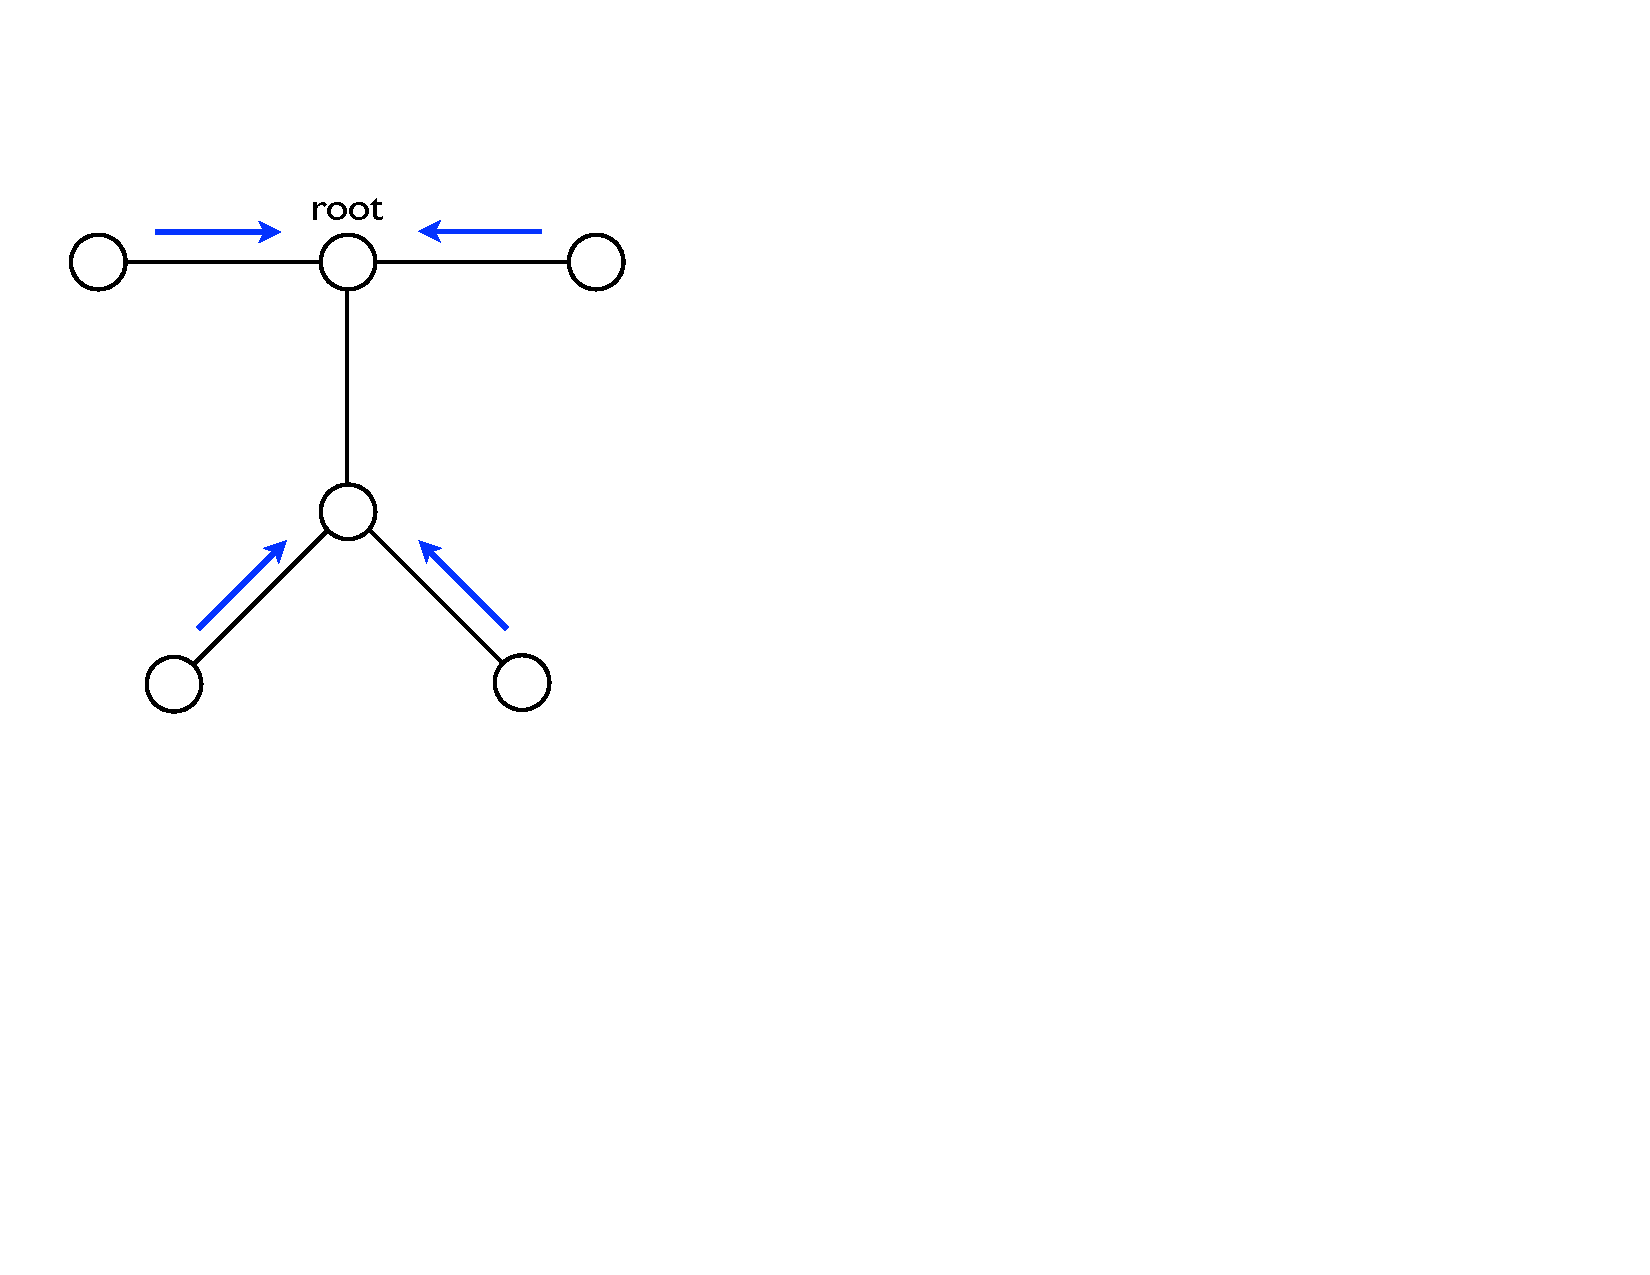
\includegraphics[width=0.20\linewidth]{figures/graphical_models/rootman1.pdf}}
\sublabel{b}{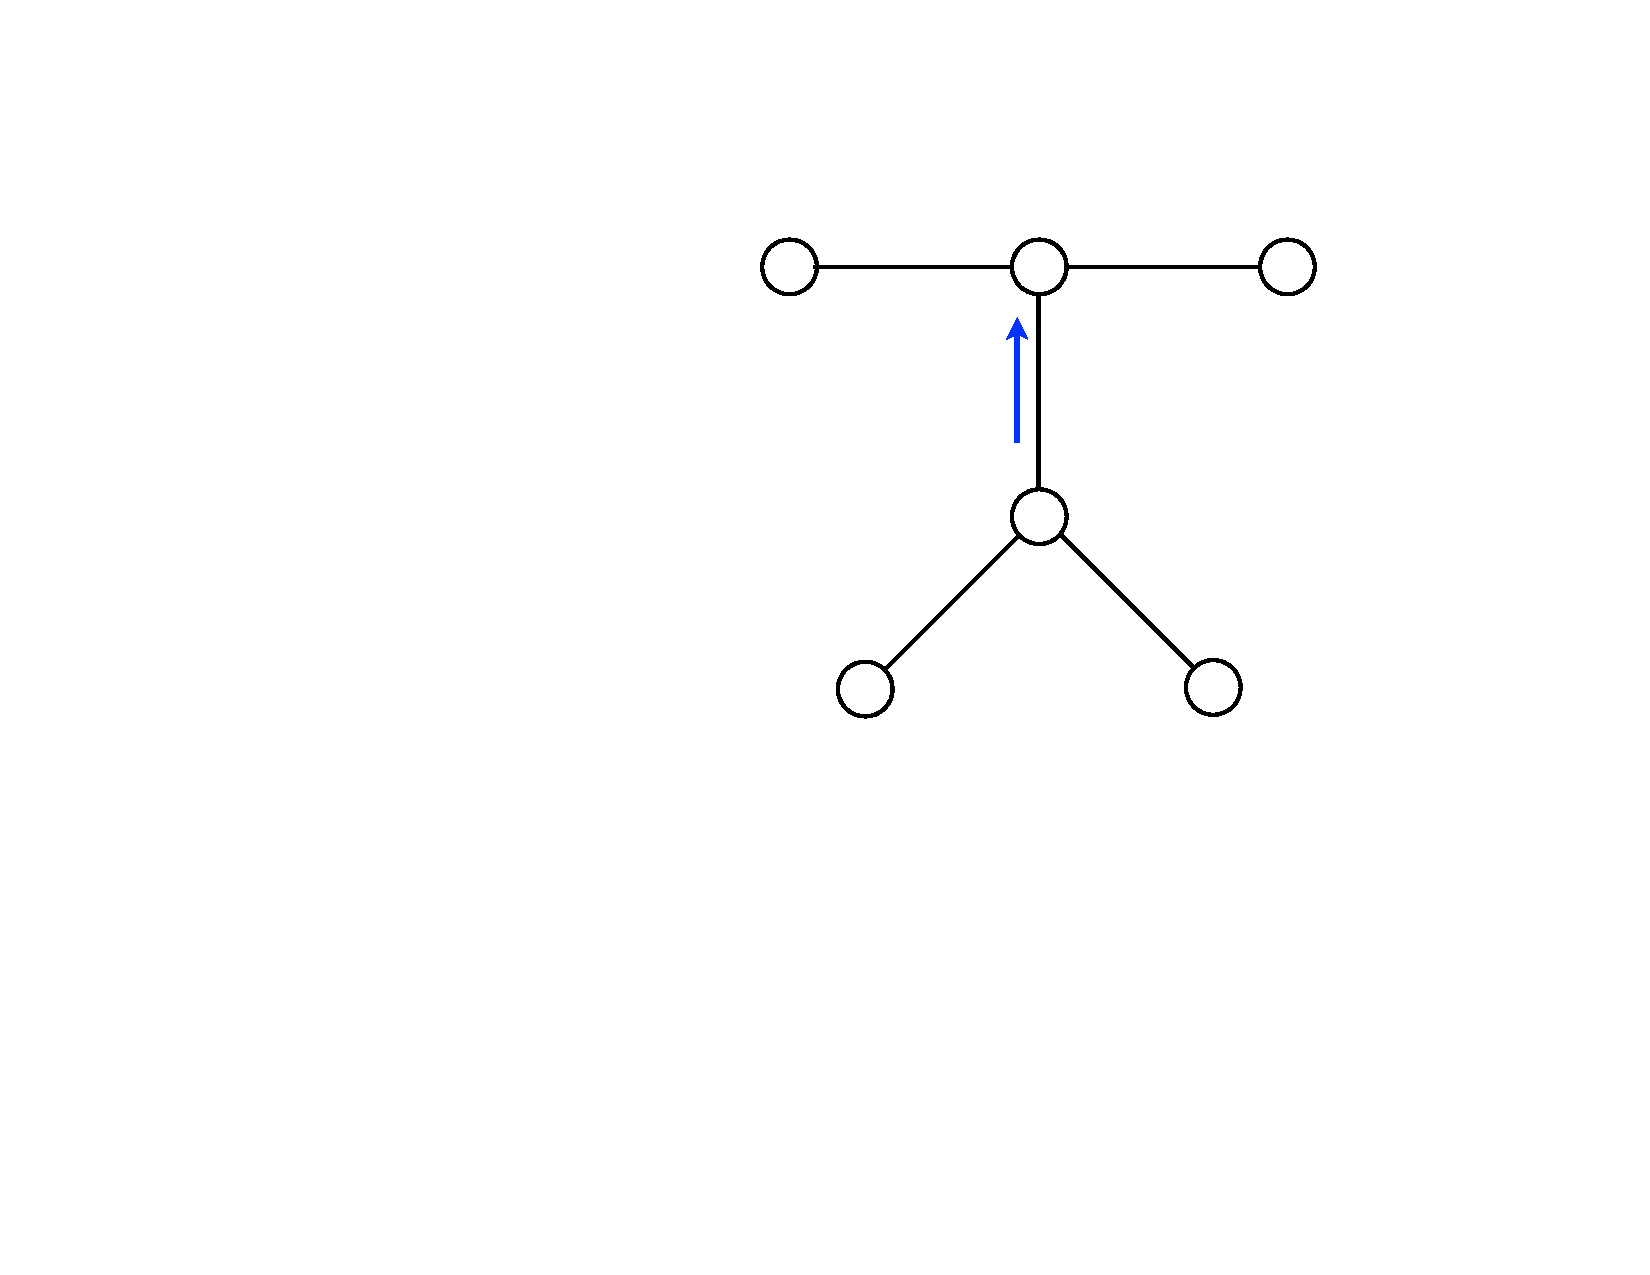
\includegraphics[width=0.20\linewidth]{figures/graphical_models/rootman2.pdf}}
\sublabel{c}{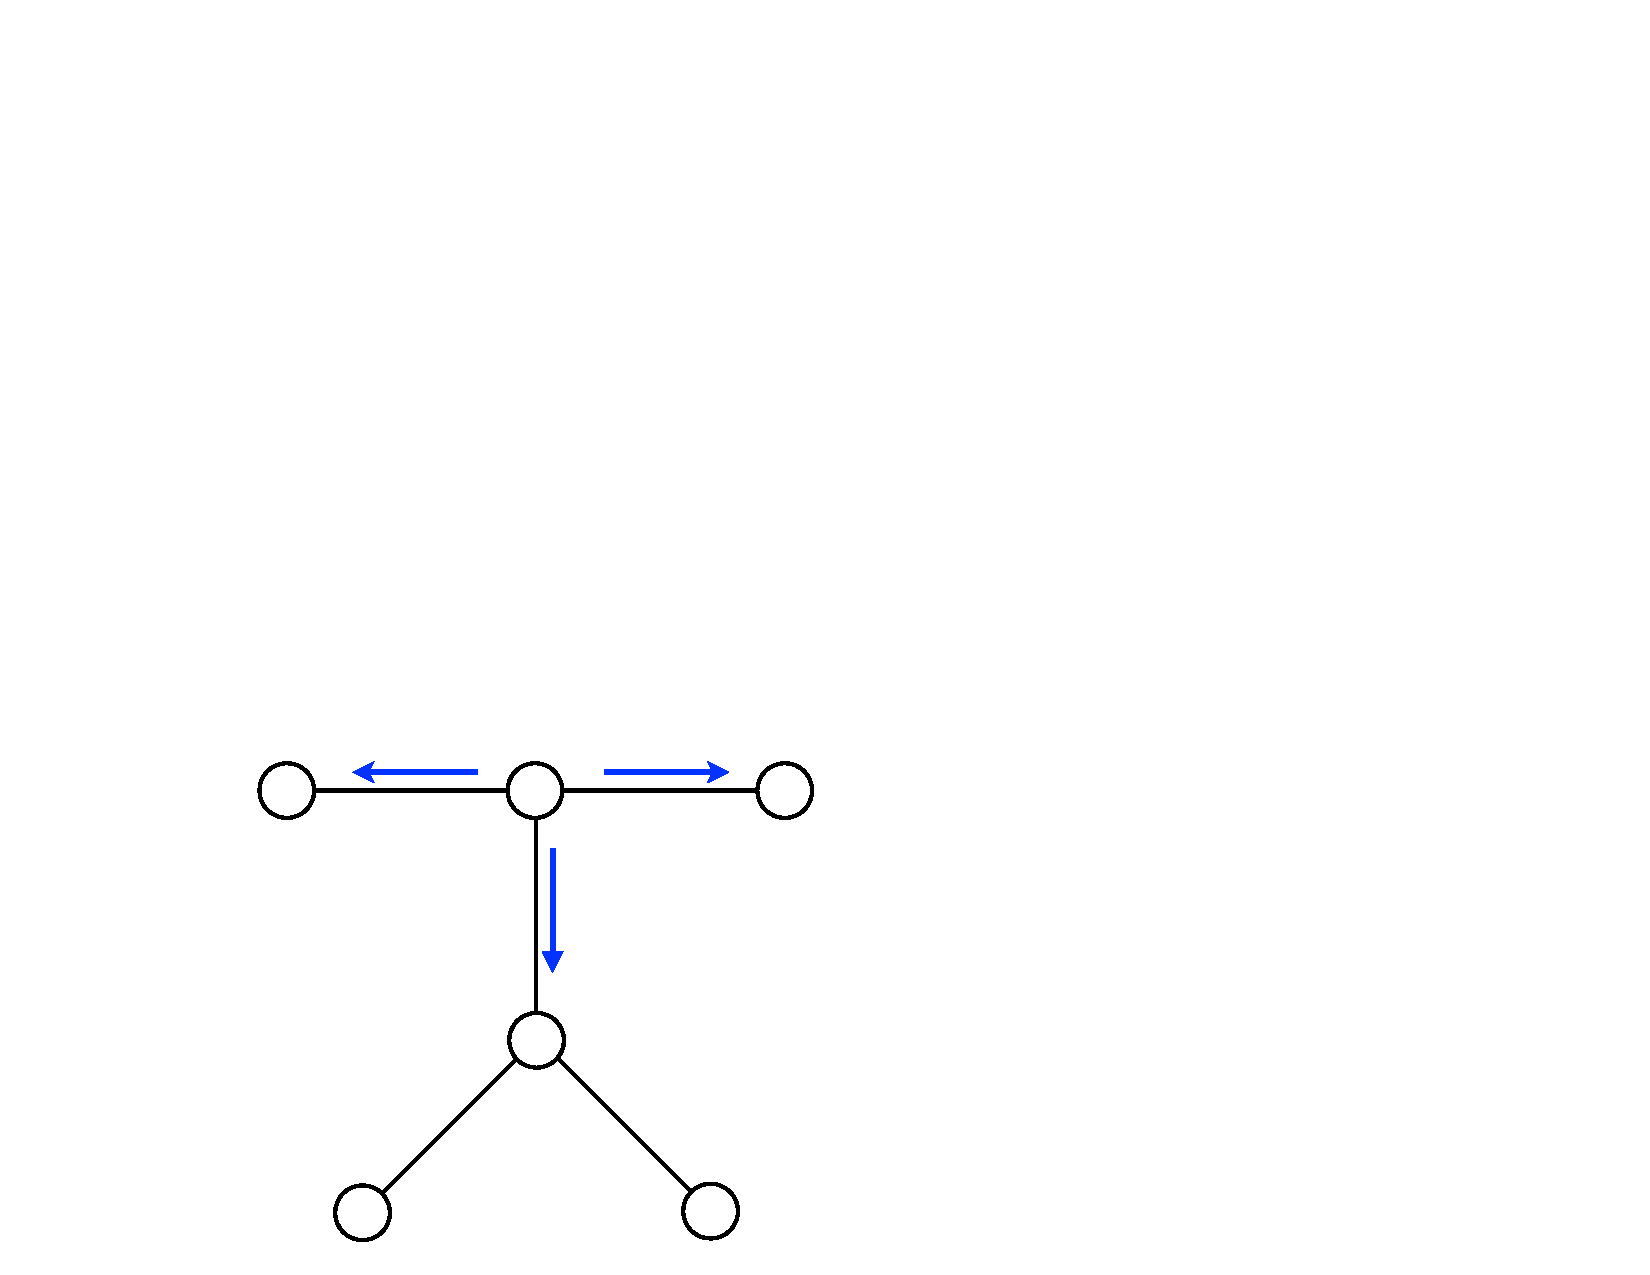
\includegraphics[width=0.20\linewidth]{figures/graphical_models/rootman3.pdf}}
\sublabel{e}{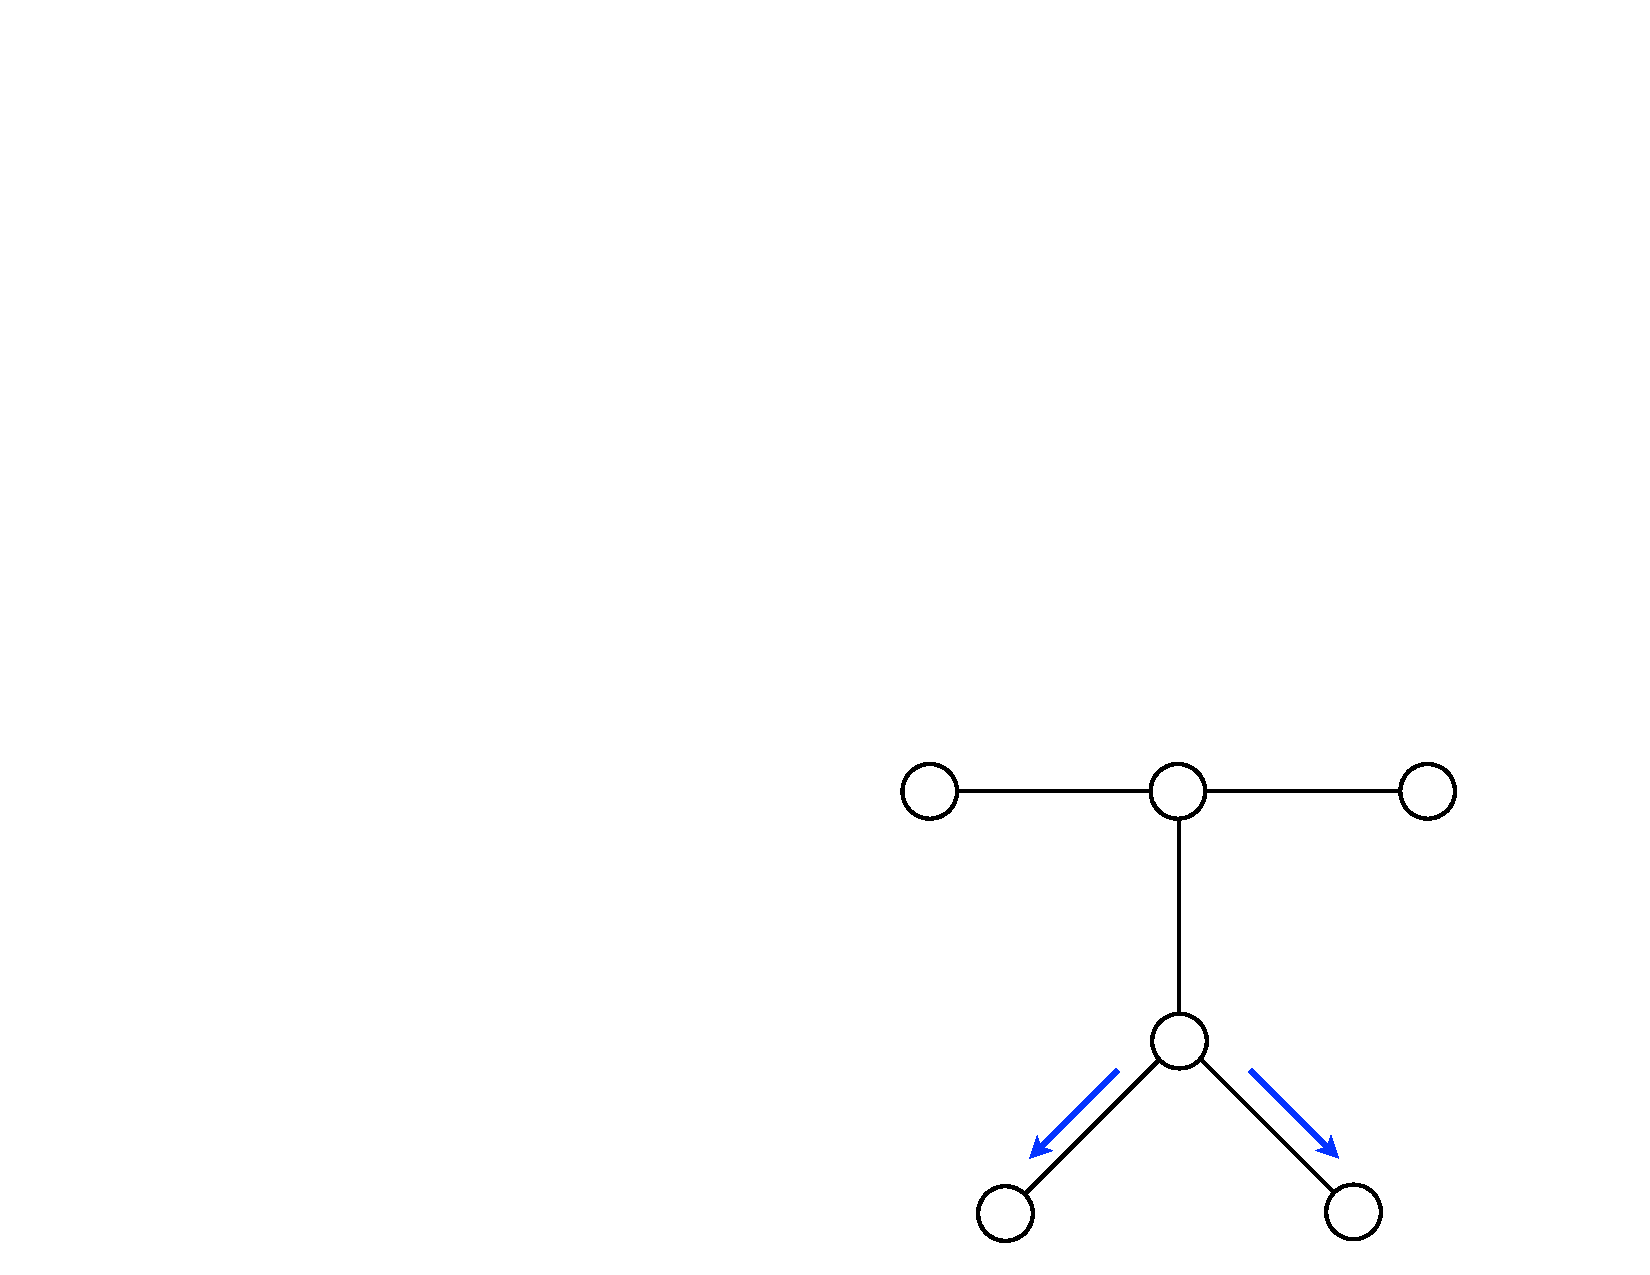
\includegraphics[width=0.20\linewidth]{figures/graphical_models/rootman4.pdf}}
}
\caption{Example of a {\bf depth-first update schedule} for BP
  message passing.  We arbitrarily select one node as the root.
(a) Messages begin at the leaves and (b) proceed to the root.  Once
all the messages reach the designated root node, (c) an outgoing sweep
computes the remaining messages, (d) ending at the leaf nodes.}
\label{fig:men2}
\end{figure}

\subsection{Example belief propagation application: stereo}

Assume that we want to compute the depth from a stereo image pair, such as the pair shown in (a) and (b) in Fig.~\ref{fig:canoe1}, and with their insets marked with the red rectangles, shown in (c) and (d).   Assume that the two images have been rectified, as described in Chapter (stereo), and consider the common scanline, marked in each of (c) and (d) with a black horizontal line.  The luminance intensities of each scanline are plotted in Fig.~\ref{fig:canoe2}.  Most computer vision stereo algorithms \cite{Scharstein2002} examine multiple scanlines to compute the depth at every pixel, but to illustrate a simple example of belief propagation in vision, we will consider the stereo vision problem while considering only one scanline pair at a time.

The graphical model that describes this stereo depth reconstruction for a single scanline is shown in Fig.~\ref{fig:canoe3}.  Each unfilled circle in the graphical models represents the unknown depth of each pixel in the scan line of one of the stereo images, in this example, the left camera image in Fig.~\ref{fig:canoe1}, (c).  The open circles mean that the depth of each pixels is an unobserved variable.  

The intensity values of the left and right camera scan lines are used to compute the local evidence for the disparity offset, $d[i, j]$, of each right camera pixel corresponding to the left image pixel at each right camera position, $[i,j]$.  For this example, we assume that each right camera pixel value, $x_r$ is that of a corresponding left camera value, $x_l$, but with independent, identically distributed (IID) Gaussian random noise added.  This leads to a simple formula for the local evidence, $\psi_i$, for the given depth value of any pixel,
\begin{equation}
    \psi_i = P(d[i,j] | x_r, x_l) =  k e^{-\sum_{i=-10}^{i=10} \frac{(x_r[i,j] - x_l[i - d[i, j], j])^2}{2 \sigma^2}  }
\end{equation}
For simplicity in this example, we discretize the $x_r$ to $x_l$ disparity offset into 4 different bins, each 45 disparity offsets wide.  For simplicity, we add the local disparity evidence over the 45 depth states, then normalize the sum at each $n$ to maintain a probability distribution.  The resulting local evidence matrix, for each of the 4 depth states, at each left camera spatial position, is displayed in the 3rd row of Fig.~\ref{fig:canoe4}.  The intensities in each column in the third-row image add-up to one.

The prior probability of any configuration of pixel disparity states is described by setting the compatibility matrices, $\mathbf{\phi}[s_i, s_{i+1}]$ of the Markov chain of Fig.~\ref{fig:canoe3}.  For this example, we use a compatibility matrix referred to as the Potts Model \cite{Wu1982}:
\begin{equation}
  \mathbf{\phi}[s_i, s_{i+1}] = 
    \begin{cases}
      1, & \text{if}\ s_i = s_{i+1} \\
      \delta, & \text{otherwise}
    \end{cases}
\end{equation}
For this example, we used $\delta = 0.001$

We then ran BP, Eq.~\ref{eq:bpupdate} in a depth-first update schedule.  For this network, that involves two linear sweeps over all the nodes of the chain, first from left to right, then from right to left.  Starting from the left-most node, we updated the rightward messages one node at a time, in a rightward sweep, then, starting from the right-most node, updated all the leftward messages one node at a time, in a leftward sweep.

Once all the messages were computed, we used Eq.~\ref{eq:bpmarginal} to find the posterior marginal probability at each node.  The local evidence, the leftward and rightward messages, and the final marginal probability at each node are displayed for every left-camera pixel of the inset.  The four rows of each display in subimages (c)-(f) correspond to the four possible depth states used for this calculation. 
Note that for this scanline, in this image pair, there is a depth discontinuity at location of the red vertical mark in Fig.~\ref{fig:canoe4}--the canoe is closer to the camera than the ground beyond the canoe that appears to the right of the canoe.  The local evidence for depth disparity, (c), is rather inaccurate, but the marginal posterior probability accurately finds the depth discontinuity at the canoe boundary.

\begin{figure}
\centerline{
\sublabel{a}{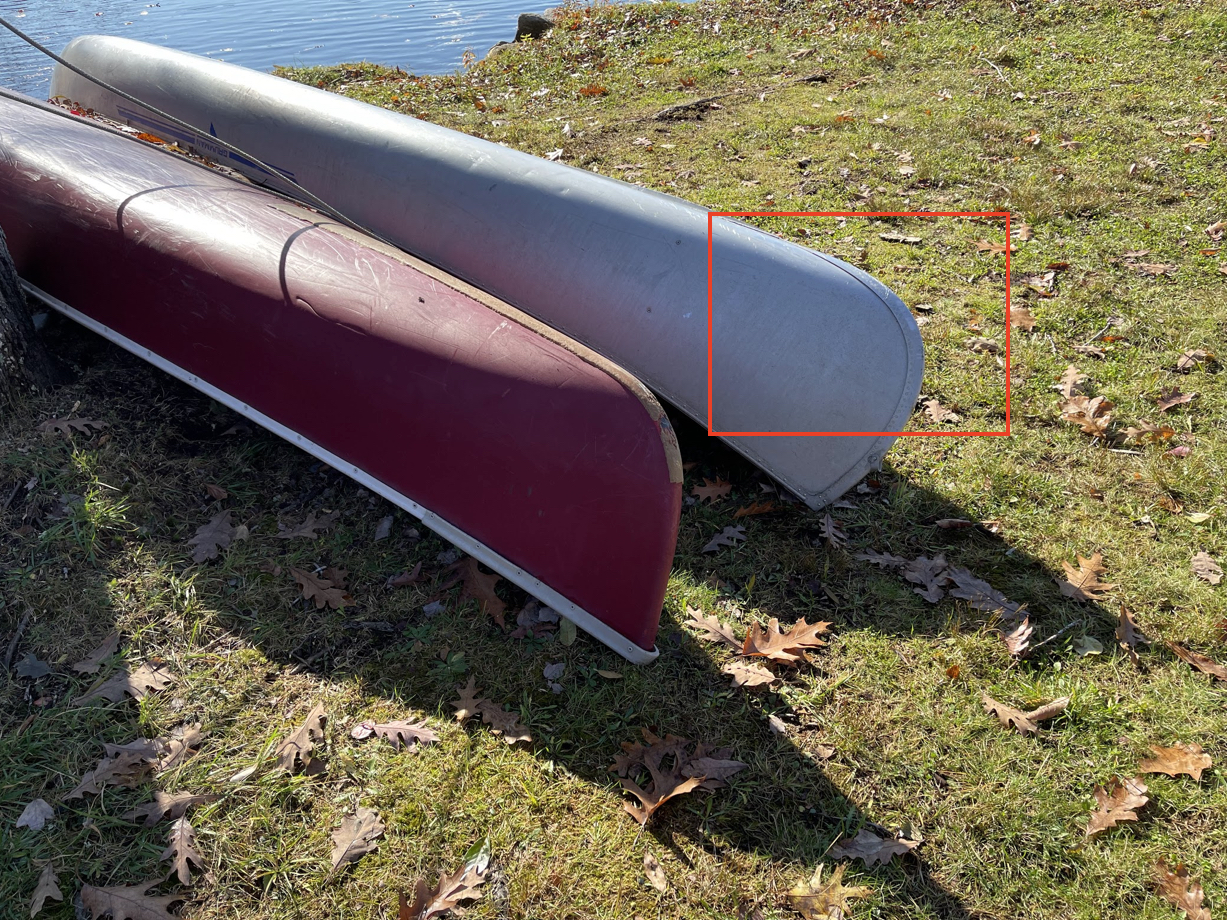
\includegraphics[width=0.40\linewidth]{figures/graphical_models/lcanoebig.jpg}}
\sublabel{b}{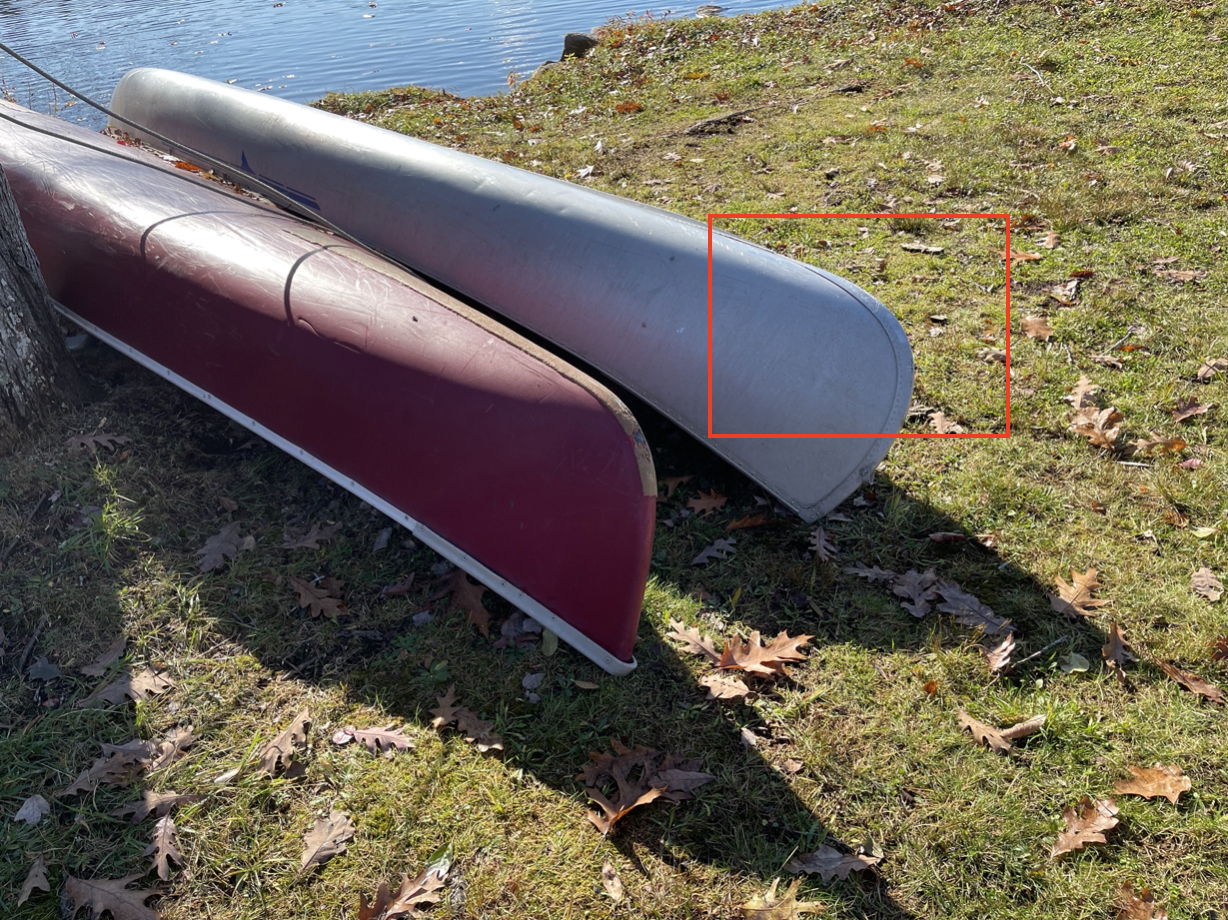
\includegraphics[width=0.40\linewidth]{figures/graphical_models/rcanoebig.jpg}}
}
\centerline{
\sublabel{c}{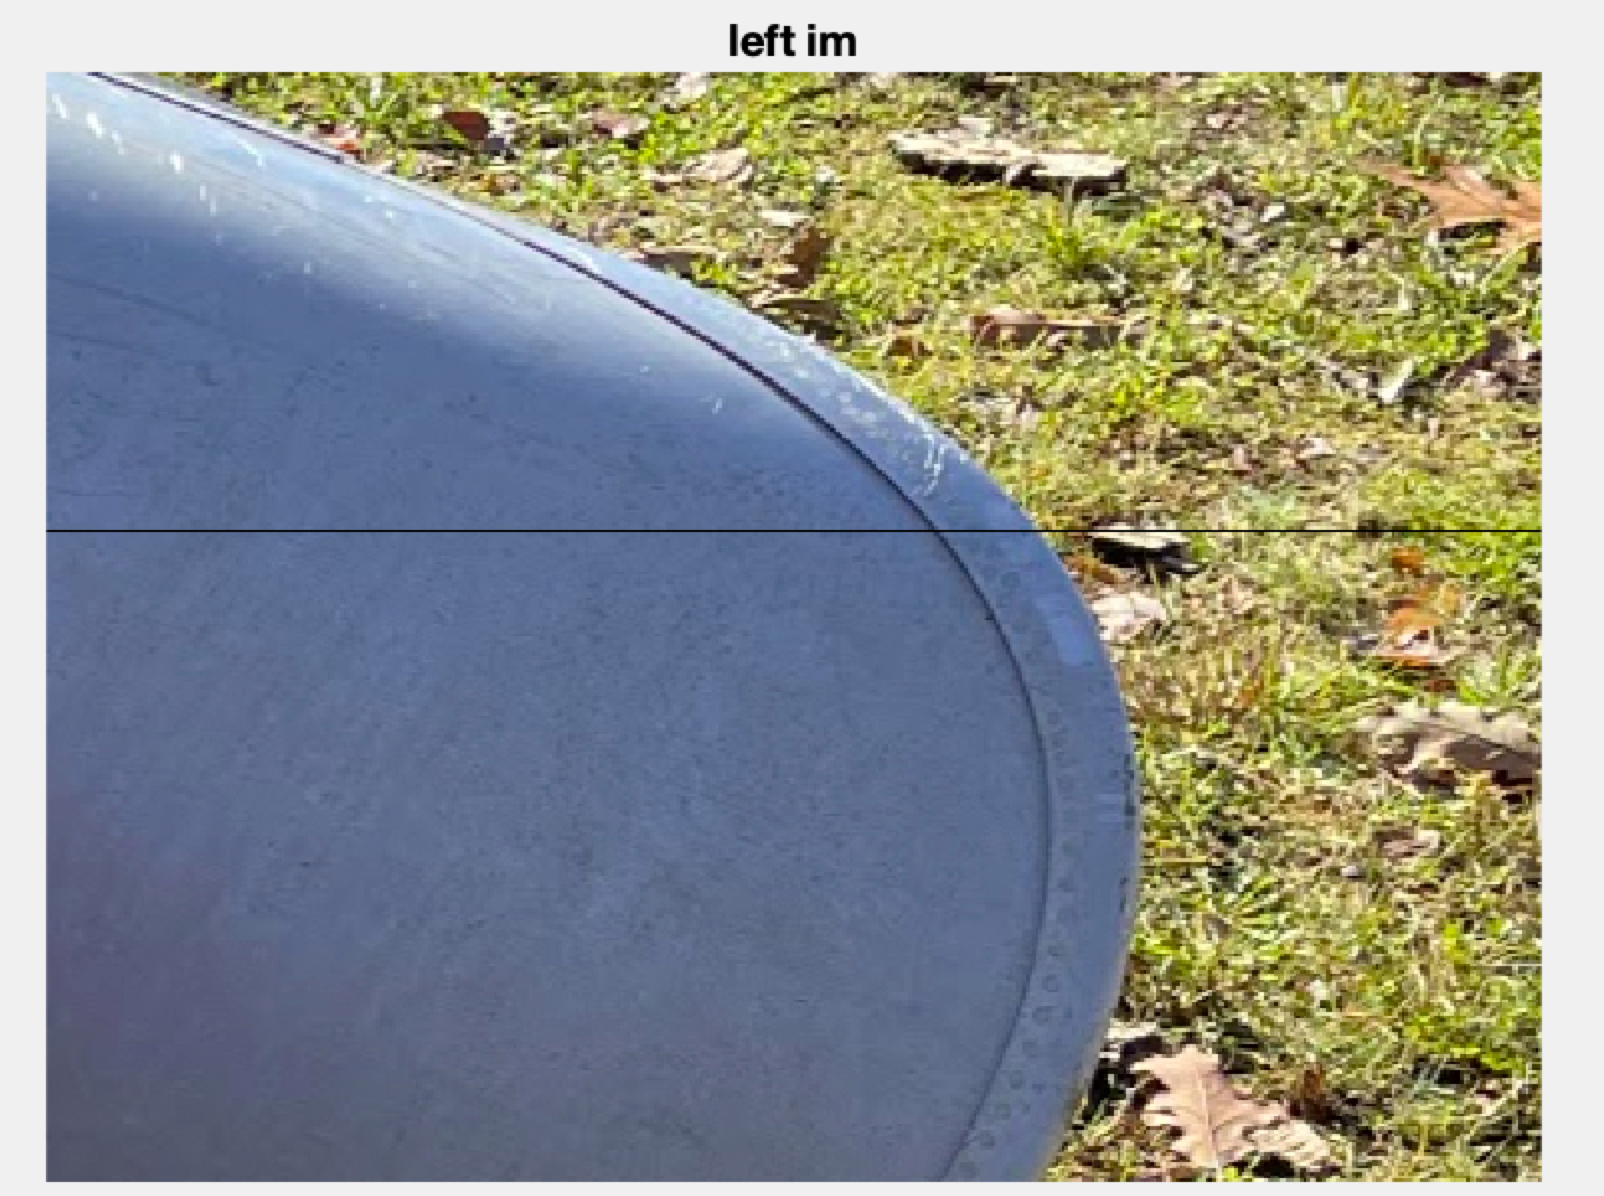
\includegraphics[width=0.40\linewidth]{figures/graphical_models/lcanoe.jpg}}
\sublabel{d}{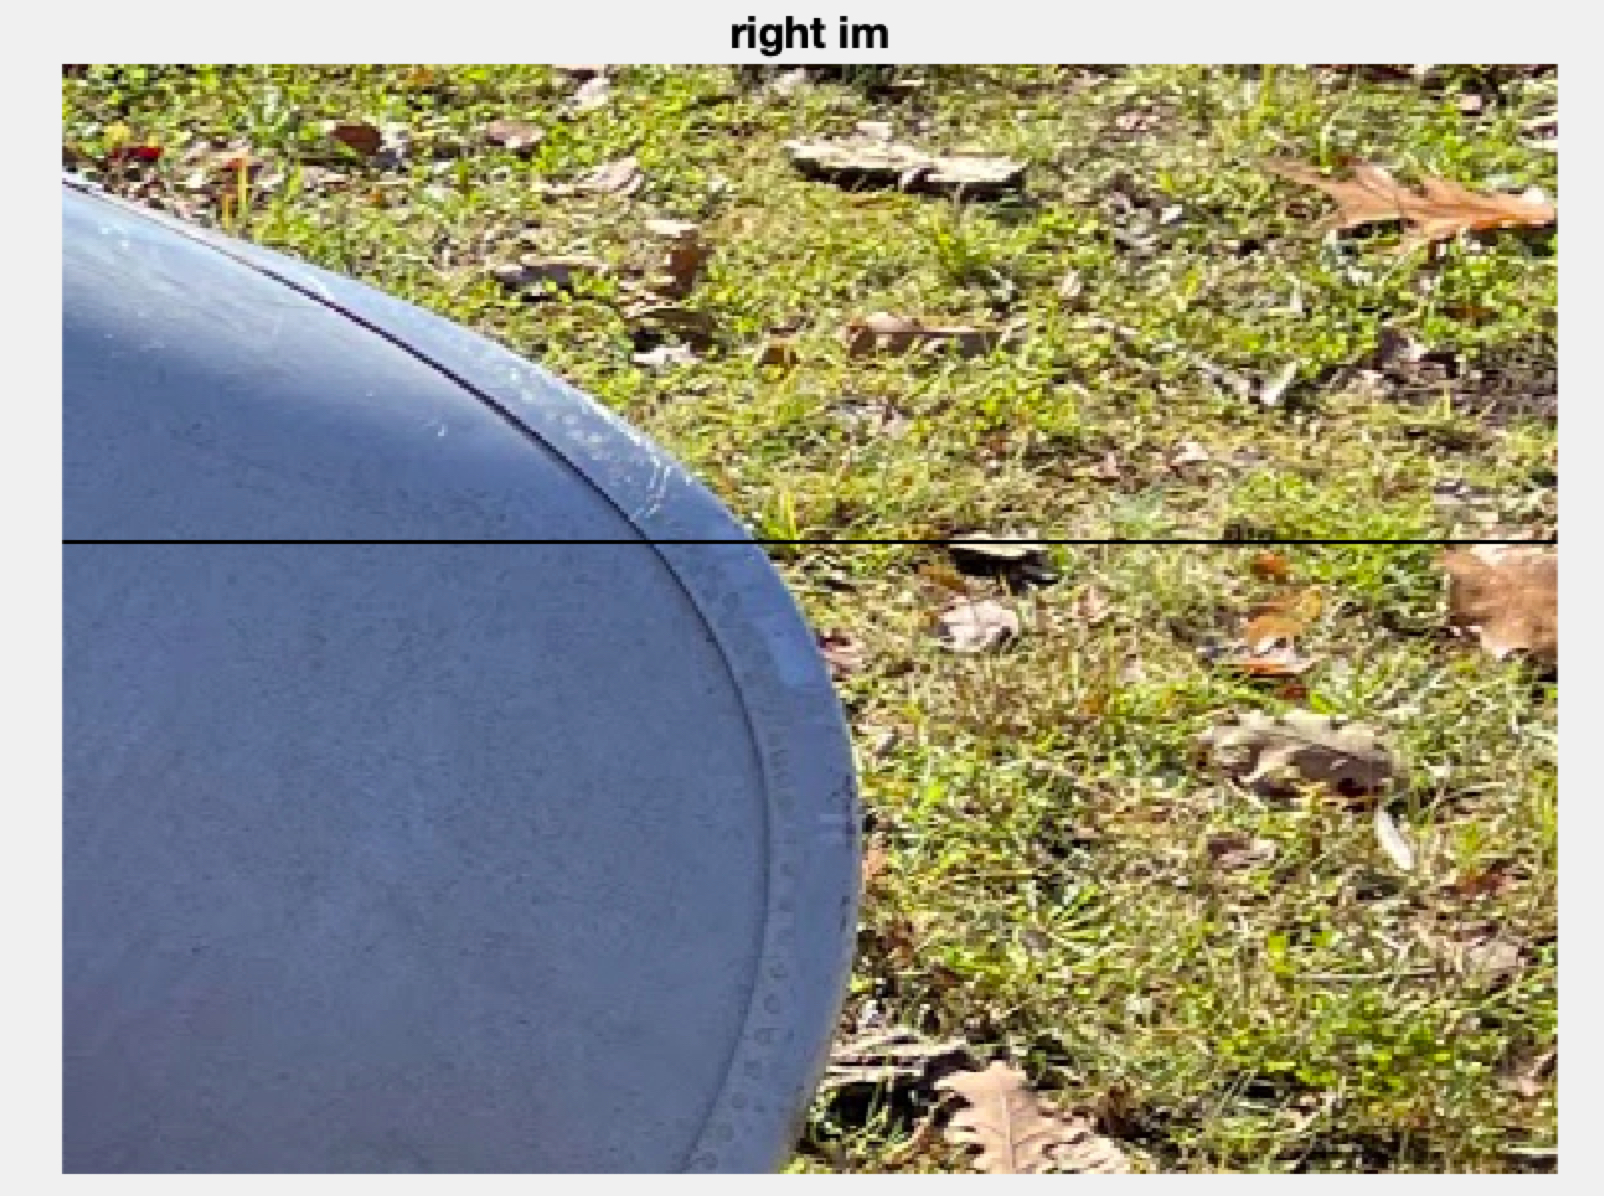
\includegraphics[width=0.40\linewidth]{figures/graphical_models/rcanoe.jpg}}
}
\caption{(a) left camera image and (b) right camera image. (c) and (d): insets showing areas of analysis.}
\label{fig:canoe1}
\end{figure}

\begin{figure}
\centerline{
\sublabel{a}{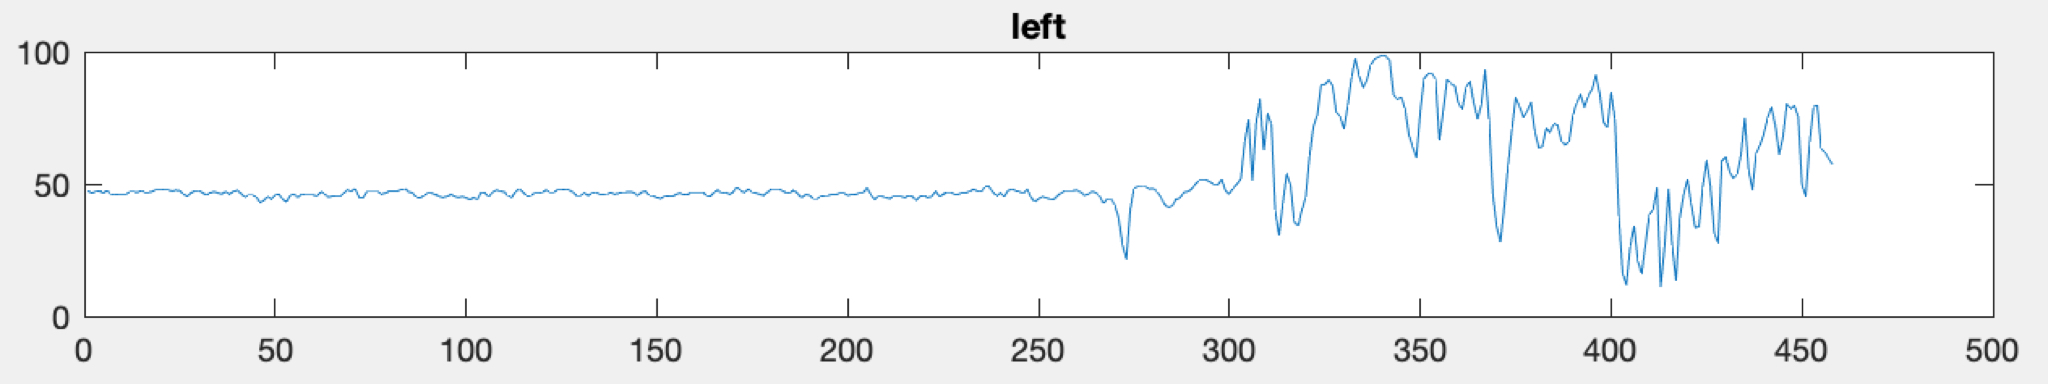
\includegraphics[width=0.80\linewidth]{figures/graphical_models/lcanoeline.jpg}}}
\centerline{
\sublabel{b}{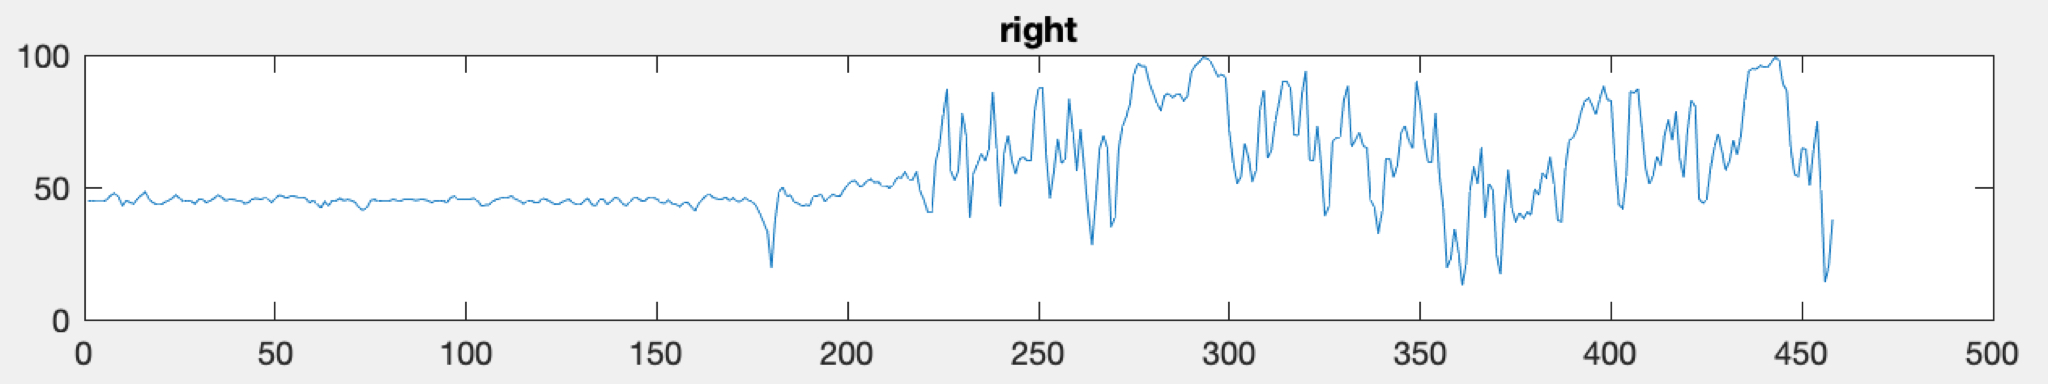
\includegraphics[width=0.80\linewidth]{figures/graphical_models/rcanoeline.jpg}}
}
\caption{(a) and (b) show the luminance traces from the scanlines marked in black in Fig.~\ref{fig:canoe1}~(c) and (d), respectively.}
\label{fig:canoe2}
\end{figure}

\begin{figure}
\centerline{
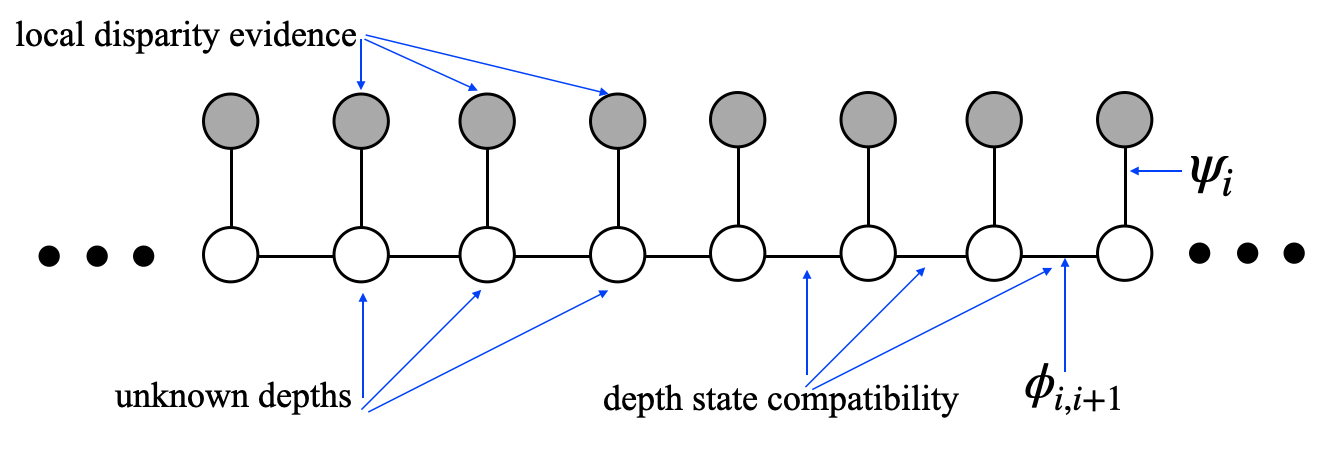
\includegraphics[width=0.80\linewidth]{figures/graphical_models/stereomodel2.jpg}
}
\caption{Graphical model for the posterior probability for stereo disparity offset between the left and right camera views from a stereo rig.}
\label{fig:canoe3}
\end{figure}

\begin{figure}
\centerline{
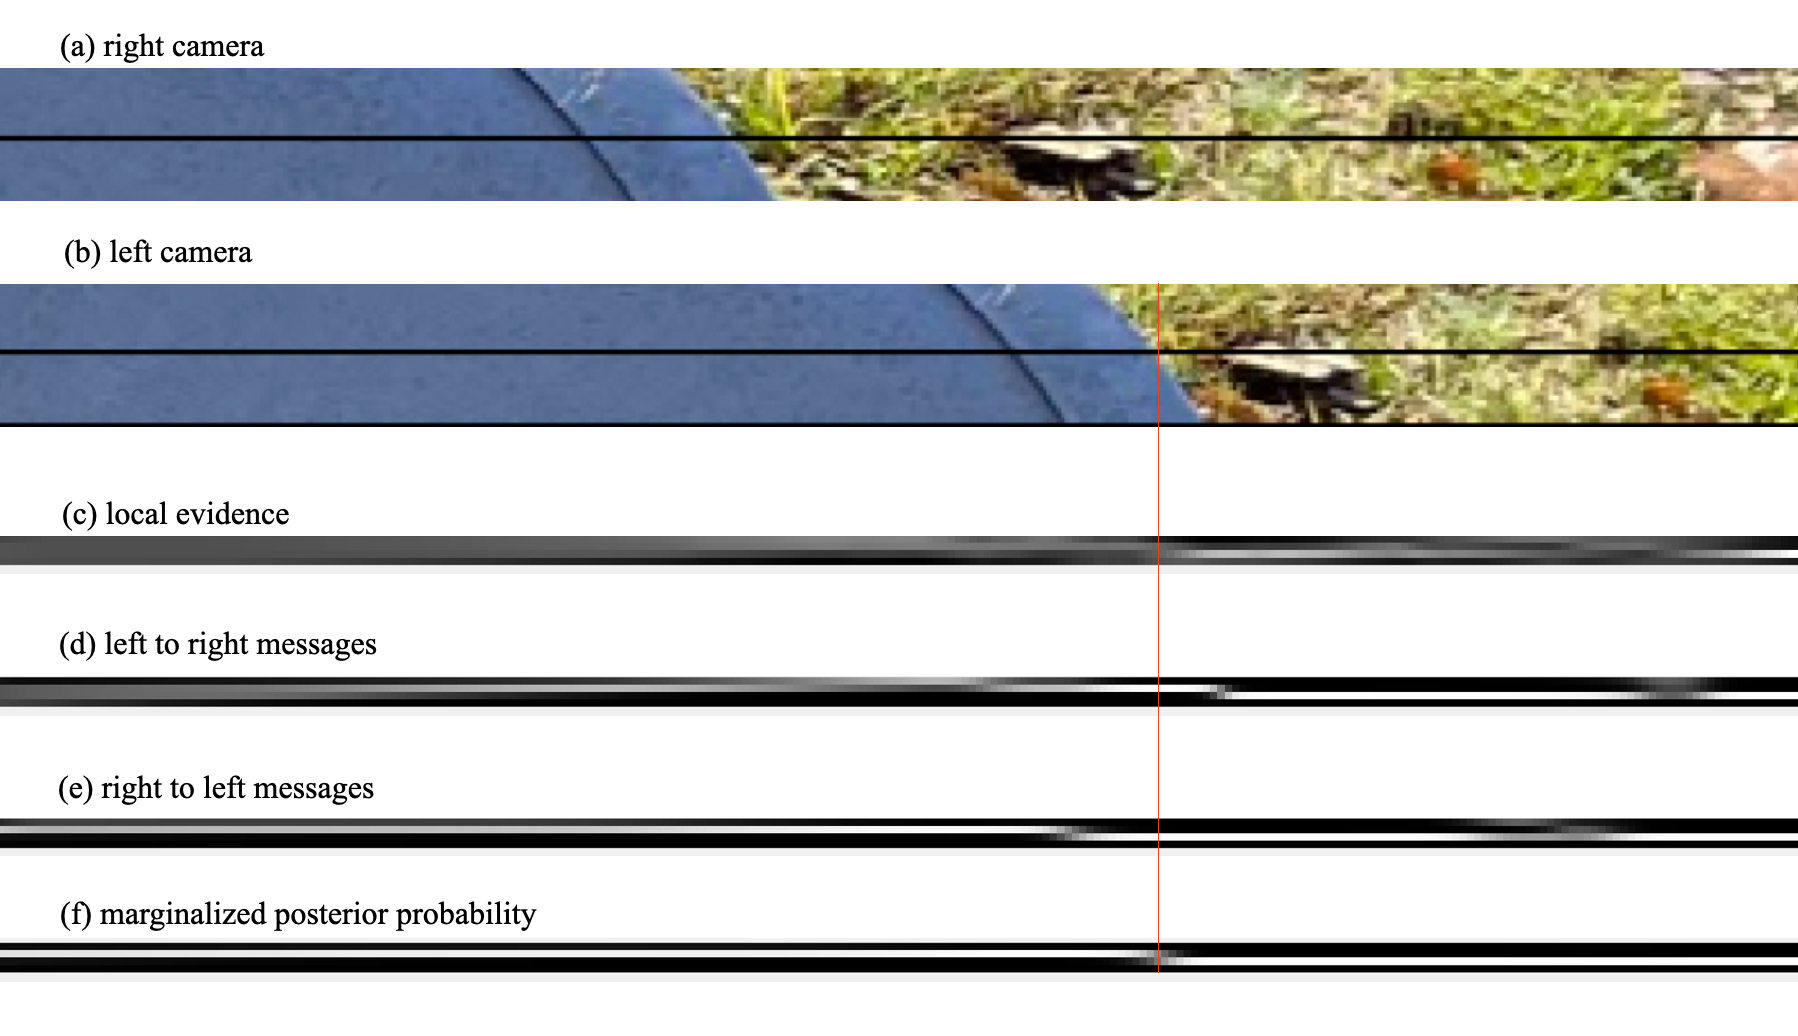
\includegraphics[width=1.0\linewidth]{figures/graphical_models/bpcanoes2.jpg}
}
\caption{Belief propagation applied to graphical model, Fig.~\ref{fig:canoe3}, for the stereo problem. (a) and (b): left and right camera views.  The luminance values covered by the black line in each figure is the stereo observation for this example.  (c) is the average over a depth range of the local evidence for a given depth offset disparity.  (d) and (e) show the local messages computed in the belief propagation algorithm at each position.  (f) shows the final marginalized posterior probability at each pixel of the left camera.  Note that the belief propagation algorithm accurately finds the position of the depth discontinuity.}
\label{fig:canoe4}
\end{figure}


\section{Loopy belief propagation}

The BP message update rules only work to give the exact marginals when
the topology of the network is that of a tree or a chain.   In general, one can show that exact
computation of marginal probabilities for graphs with loops depends on
a graph-theoretic quantity known as the treewidth of the graph.  For
many graphical models of interest in vision, such as 2-d Markov Random
Fields related to images, these quantities can be intractably large.

But the
message update rules are described locally, and one might imagine that
it is a useful local operation to perform, even without the global
guarantees of ordinary BP.   It turns out that is true.   Here is the algorithm:
{\bf loopy belief propagation algorithm}
\begin{enumerate}
\item convert graph to pairwise potentials
\item initialize all messages to all ones, or to random values
 between 0 and 1.
\item  run the belief propagation update rules of
  Sect.~\ref{sect:bpRules} until convergence.
\end{enumerate}

One can show that, in networks with loops, fixed points of the
belief propagation algorithm (message configurations where the
messages don't change with a message update) correspond to minima of a
well-known approximation from the statistical physics community known 
as the Bethe free energy \cite{Yedidia00b}.  In practice, the solutions found by the loopy belief propagation algorithm are often quite good \cite{Murphy1999}.
%, and other algorithms in this vein have been developed which are better still \cite{Wainwright03}.


\section{MAP estimation and energy models}

Instead of summing over the states of other nodes, we are sometimes
interested in finding the $\mathbf{x}$ that maximizes the joint probability.  The argmax
operator passes through constant variables just as the summation sign
did.  This leads to an alternate version of the belief propagation
algorithm, Eq.~(\ref{eq:bpupdate}), with the summation (of multiplying the vector message products by the node compatibility matrix) replaced with ``argmax''.  This is
called the ``max-product'' version of belief propagation, and it
computes an MAP estimate of the hidden states.   

Improvements have been developed over loopy belief propagation for the
case of MAP estimation, see, for example, tree-reweighted belief propagation \cite{Kolmogorov2006} and graph cuts \cite{Zabih2004}.


\subsection{Numerical example of Belief Propagation}
\label{sect:numerical}

Here we work though a numerical example of belief propagation.  To make the arithmetic easy,
we'll solve for the marginal probabilities in the graphical model of
two-state (0 and 1) random variables shown in Fig.~\ref{fig:numerical}.  That
graphical model has 3 hidden variables, and one variable observed to
be in state 0.  The compatibility matrices are given in the arrays
below (for which the state indices are 0, then 1, reading from left to
right and top to bottom).
\begin{equation}
\psi_{12}(x_1, x_2) = 
\left( 
\begin{array}{cc}
1.0 & 0.9 \\
0.9 & 1.0 
\end{array}
\right)
\end{equation}

\begin{equation}
\psi_{23}(x_2, x_3) = 
\left( 
\begin{array}{cc}
0.1 & 1.0 \\
1.0 & 0.1 
\end{array}
\right)
\end{equation}

\begin{equation}
\psi_{42}(x_2, y_2) = 
\left( 
\begin{array}{cc}
1.0 & 0.1 \\
0.1 & 1.0 
\end{array}
\right)
\end{equation}

\begin{figure}
\centerline{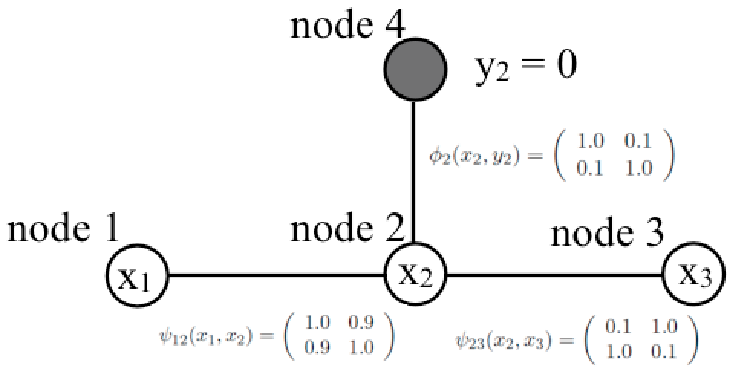
\includegraphics[width=0.48\linewidth]{figures/graphical_models/numerical.pdf}} 
\caption{Undirected graphical model used in belief propagation example} 
\label{fig:numerical}
\end{figure}
Note that in defining these potential functions, we haven't taken care to normalize the joint probability, so
we'll need to normalize each marginal probability at the end.
(remember $P(x_1,
x_2, x_3, y_2) = \psi_{42}(x_2, y_2) \psi_{23}(x_2, x_3) \psi_{12}(x_1,
x_2)$, which should sum to 1 after summing over all states.)


For this simple toy example, we can tell what results to expect by inspection, then verify that BP is doing the right thing.  Node $x_2$ wants very much to look like $y_2=0$, because
$\psi_{42}(x_2, y_2)$ contributes a large valued to the posterior
probability when $x_2 = y_2 = 1$ or when $x_2 = y_2 = 0$.  From
$\psi_{12}(x_1, x_2) $ we see that
$x_1$ has a very mild preference to
look like $x_2$.  So we expect the marginal probability at node $x_2$
will be heavily biased toward $x_2=0$, and that node $x_1$ will have a
mild preference for state 0.  $\psi_{23}(x_2, x_3)$ encourages 
$x_3$ to be the opposite of $x_2$, so it will be biased toward the state $x_3=1$.

Let's see what belief propagation gives.  We'll
follow the parallel, synchronous update scheme for calculating
all the messages.  The leaf nodes can send messages along their
edges without waiting for any messages to be updated.  For the message
from node 1, we have
\begin{eqnarray} 
m_{12}(x_2) & = & \sum_{x_1} \psi_{12} (x_1, x_2)  \\
& = & 
\left( 
\begin{array}{cc} 
1.0 & 0.9 \\ 
0.9 & 1.0 
\end{array}
\right) 
\left( 
\begin{array}{c} 
1 \\ 
1
\end{array}
\right) 
 \\
& = &
\left( 
\begin{array}{c} 
1.9 \\ 
1.9
\end{array}
\right) \\
&  = &
k
\left( 
\begin{array}{c} 
1 \\ 
1
\end{array}
\right) 
\end{eqnarray} 
For numerical stability, we typically normalize the computed messages in Eq.~(\ref{eq:bpupdate}) so
the entries sum to 1, or so their maximum entry is 1, then remember
to renormalize the final marginal probabilities to sum to 1.
Here, we've normalized the messages for simplicity, (absorbing the
normalization into a constant, k).

The message from node 3 to node 2 is
\begin{eqnarray}
m_{32}(x_2) & = & \sum_{x_3} \psi_{32} (x_2, x_3)  \\
& = & 
\left( 
\begin{array}{cc}
0.1 & 1.0 \\
1.0 & 0.1 
\end{array}
\right) 
\left( 
\begin{array}{c} 
1 \\ 
1
\end{array}
\right) 
 \\
& = &
\left( 
\begin{array}{c}
1.1 \\
1.1
\end{array}
\right) \\
&  = &
k
\left( 
\begin{array}{c}
1 \\
1
\end{array}
\right) 
\end{eqnarray}

We have a non-trivial message from observed node $y_2$ (node 4) to the hidden
variable $x_2$:
\begin{eqnarray}
m_{42}(x_2) & = & \sum_{x_4} \psi_{42} (x_2, y_2)  \\
& = & 
\left( 
\begin{array}{cc}
1.0 & 0.1 \\
0.1 & 1.0 
\end{array}
\right)  
\left( 
\begin{array}{c}
1 \\
0
\end{array}
\right) 
\\
& = &
\left( 
\begin{array}{c}
1.0 \\
0.1
\end{array}
\right) 
\end{eqnarray}
where $y_2$ has been fixed to $y_2 = 0$, thus restricting $\psi_{42}
(x_2, y_2) $ to just the first column.

Now we just have two messages left to compute before we have all
messages computed (and therefore all node marginals computed from
simple combinations of those messages).  
The message from node 2 to node 1 uses the messages from nodes 4 to 2
and 3 to 2:
\begin{eqnarray}
m_{21}(x_1) & = & \sum_{x_2} \psi_{12} (x_1, x_2)  m_{42}(x_2) m_{32}(x_2) \\
& = & 
\left( 
\begin{array}{cc}
1.0 & 0.9 \\
0.9 & 1.0 
\end{array}
\right) 
\left[
\left( 
\begin{array}{c}
1.0 \\
0.1
\end{array}
\right) 
.*
\left( 
\begin{array}{c}
1 \\
1
\end{array}
\right) 
\right]
=
\left( 
\begin{array}{c}
1.09 \\
1.0
\end{array}
\right) 
\end{eqnarray}

The final message is that from node 2 to node 3 (since $y_2$ is
observed, we don't need to compute the message from node 2 to node
4).  That message is:
\begin{eqnarray}
m_{23}(x_3) & = & \sum_{x_2} \psi_{23} (x_2, x_3)   m_{42}(x_2) m_{12}(x_2) \\
& = & 
\left( 
\begin{array}{cc}
0.1 & 1.0 \\
1.0 & 0.1 
\end{array}
\right) 
\left[
\left( 
\begin{array}{c}
1.0 \\
0.1
\end{array}
\right) 
.*
\left( 
\begin{array}{c}
1 \\
1
\end{array}
\right) 
\right]
=
\left( 
\begin{array}{c}
0.2 \\
1.01
\end{array}
\right) 
\end{eqnarray}

Now that we've computed all the messages, let's look at the marginals
of the three hidden nodes.  The product of all the messages arriving
at node 1 is just the one message, $m_{21}(x_1)$, so we have
(introducing constant k to normalize the product of messages to be a
probability distribution)
\begin{equation}
P_1(x_1) = k m_{21}(x_1) 
=
\frac{1}{2.09}
\left( 
\begin{array}{c}
1.09 \\
1.0
\end{array}
\right) 
\end{equation}
As we knew it should, node 1 shows a slight preference for state 0.

The marginal at node 2 is proportional to the product of 3 messages.
Two of those are trivial messages, but we'll show them all for
completeness:
\begin{eqnarray}
P_2(x_2) & = & k m_{12}(x_2)  m_{42}(x_2)  m_{32}(x_2) \\
& = & k 
\left( 
\begin{array}{c} 
1 \\ 
1
\end{array}
\right) 
.*
\left( 
\begin{array}{c}
1.0 \\
0.1
\end{array}
\right) 
.* 
\left( 
\begin{array}{c} 
1 \\ 
1
\end{array}
\right) \\
& = &
\frac{1}{1.1}
\left( 
\begin{array}{c}
1.0 \\
0.1
\end{array}
\right) 
\end{eqnarray}
As expected, belief propagation reveals a strong bias for node 2 being in state 0.

Finally, for the marginal probability at node 3, we have
\begin{equation}
P_3(x_3) = k m_{23}(x_3) 
=
\frac{1}{1.21}
\left( 
\begin{array}{c}
0.2 \\
1.01
\end{array}
\right) 
\end{equation}
As predicted, this variable is biased toward being in state 1.

By running belief propagation within this tree, we have computed the
exact marginal probabilities at each node, reusing the intermediate
sums across different marginalizations, and exploiting the structure
of the joint probability to perform the computation efficiently.  If
nothing were known about the joint probability structure, the
marginalization cost would grow exponentially with the number of nodes
in the network.  But if the graph structure corresponding to the joint
probability is known to be a chain or a tree, then the marginalization
cost only grows linearly with the number of nodes, and is quadratic in
the node state dimensions.  The belief propagation algorithm enables inference in many large-scale problems.

\begin{comment}

https://www.cs.cmu.edu/~epxing/Class/10708-15/notes/10708_scribe_lecture25.pdf


wonderful video, with colab:
https://www.youtube.com/watch?v=8owQBFAHw7E

https://proceedings.neurips.cc/paper/2020/file/07217414eb3fbe24d4e5b6cafb91ca18-Paper.pdf    % not so interesting for the book.  Just a BPgeneralization for graph networks.

and message-passing neural networks--(summarizes a number of nn's that operate on graphs)
https://arxiv.org/pdf/1704.01212.pdf

and kipf and welling (most cited gcn):  but sort of hard to follow.
https://arxiv.org/pdf/1609.02907.pdf

and graph attention network (transformer-like):  feb 2018
https://arxiv.org/pdf/1710.10903.pdf

and:
https://thegradient.pub/transformers-are-graph-neural-networks/
This is a nice paper about composable diffusion models:
https://arxiv.org/pdf/2206.01714.pdf
\end{comment}
%% \section{graph cuts}



